\chapter{Special Analysis Procedures}
\label{ch:special}

\section{Static condensation}
A simple example: cantilever beam.
\begin{fig}
  % Cantilever beam with tip load P (static condensation example)
\begin{tikzpicture}[scale=1.0,font=\small]
  \pic at (0,0) {wallL};
  \draw[thick] (0,-0.2) rectangle (6,0.2);
  \draw[load] (6,0.3) -- (6,1.6) node[right] {$P$};
  \draw[dim] (0,-0.8) -- (6,-0.8) node[midway,fill=white,inner sep=1pt] {$L$};
  \draw (0,-0.6) -- (0,-1.0); \draw (6,-0.6) -- (6,-1.0);
\end{tikzpicture}

\end{fig}
\begin{equation*}
  \begin{bmatrix}\dfrac{12EI}{L^3} & \dfrac{-6EI}{L^2}\\[8pt] \dfrac{-6EI}{L^2} & \dfrac{4EI}{L}\end{bmatrix}\Bmat{v_2\\ \theta_2} = \Bmat{P\\ 0}
\end{equation*}
2nd Eq.: $\ -\dfrac{6EI}{L^2}v_2 + \dfrac{4EI}{L}\theta_2 = 0 \;\rightarrow\; \theta_2 = \dfrac{3v_2}{2L}$ \hfill (a)

Substitute Eq.~(a) into the 1st Eq.
\begin{gather*}
  \frac{12EI}{L^3}v_2 - \frac{6EI}{L^2}\Bigl(\frac{3v_2}{2L}\Bigr) = P \;\rightarrow\; \frac{3EI}{L^3}v_2 = P\quad\text{(Condensed system!)}\\
  \rightarrow\; v_2 = \frac{PL^3}{3EI} \;\rightarrow\; \text{(a)} \;\rightarrow\; \theta_2 = \frac{3v_2}{2L} = \frac{PL^2}{2EI}
\end{gather*}
The condensed system can be derived systematically as follows. The equations of equilibrium are
\begin{equation}
  \Kmat\bs{\Delta} = \Pvec\qquad\text{or}\qquad
  \bmat{\Kmat_{bb} & \Kmat_{bc}\\ \Kmat_{cb} & \Kmat_{cc}}\Bmat{\bs{\Delta}_b\\ \bs{\Delta}_c} = \Bmat{\Pvec_b\\ \Pvec_c}
\end{equation}
where $\bs{\Delta}_b$ are the degrees of freedom to be eliminated (condensed), $\bs{\Delta}_c$ are the remaining degrees of freedom, and $\Kmat_{cb} = \Kmat_{bc}^\tr$.

We can derive the condensed system using the following two methods.

\topic{Method 1: variable substitution}
Expand the upper partition to obtain
\begin{equation*}
  \Kmat_{bb}\bs{\Delta}_b + \Kmat_{bc}\bs{\Delta}_c = \Pvec_b
\end{equation*}
Solving for $\bs{\Delta}_b$ from the above equation, we have
\begin{equation*}
  \bs{\Delta}_b = \Kmat_{bb}^{-1}(-\Kmat_{bc}\bs{\Delta}_c + \Pvec_b)
\end{equation*}
Then by substituting $\bs{\Delta}_b$ into the lower partition, we obtain the condensed system:
\begin{equation}
  \widehat{\Kmat}_{cc}\bs{\Delta}_c = \widehat{\Pvec}_c
\end{equation}
where
\begin{equation}
  \widehat{\Kmat}_{cc} = \Kmat_{cc} - \Kmat_{cb}\Kmat_{bb}^{-1}\Kmat_{bc},\qquad
  \widehat{\Pvec}_c = \Pvec_c - \Kmat_{cb}\Kmat_{bb}^{-1}\Pvec_b
\end{equation}
Note that $\widehat{\Kmat}_{cc}$ is symmetric. Also, $\widehat{\Pvec}_c = \Pvec_c$ when $\Pvec_b = \mat{0}$.

\topic{Method 2: stationary of total potential energy}
\begin{equation}
  \bs{\Delta} = \Bmat{\bs{\Delta}_b\\ \bs{\Delta}_c} = \bmat{-\Kmat_{bb}^{-1}\Kmat_{bc}\\ \mat{I}}\bs{\Delta}_c + \Bmat{\Kmat_{bb}^{-1}\Pvec_b\\ \mat{0}} = \Tmat\bs{\Delta}_c + \mat{R}
\end{equation}
where
\begin{equation*}
  \Tmat = \bmat{-\Kmat_{bb}^{-1}\Kmat_{bc}\\ \mat{I}};\qquad \mat{R} = \Bmat{\Kmat_{bb}^{-1}\Pvec_b\\ \mat{0}}
\end{equation*}
By making use of the above equation, the strain energy in terms of $\bs{\Delta}_c$ is:
\begin{equation*}
  \begin{aligned}
    U(\bs{\Delta}) &= \tfrac12\bs{\Delta}^\tr\Kmat\bs{\Delta}\\
    &= \tfrac12(\mat{R}^\tr + \bs{\Delta}_c^\tr\Tmat^\tr)\Kmat(\Tmat\bs{\Delta}_c + \mat{R})\\
    &= \tfrac12\bs{\Delta}_c^\tr\Tmat^\tr\Kmat\Tmat\bs{\Delta}_c + \bs{\Delta}_c^\tr\Tmat^\tr\Kmat\mat{R} + \tfrac12\mat{R}^\tr\Kmat\mat{R} \equiv \widehat U(\bs{\Delta}_c)
  \end{aligned}
\end{equation*}
By definition, the load potential is
\begin{equation*}
  V(\bs{\Delta}) = -\bs{\Delta}^\tr\Pvec = -(\Tmat\bs{\Delta}_c + \mat{R})^\tr\Pvec = -\bs{\Delta}_c^\tr\Tmat^\tr\Pvec - \mat{R}^\tr\Pvec \equiv \widehat V(\bs{\Delta}_c)
\end{equation*}
where $\Pvec = \Bmat{\Pvec_b\\ \Pvec_c}$. Knowing the total potential energy $\widehat\Pi(\bs{\Delta}_c) = \widehat U + \widehat V$, the equilibrium equations can be obtained from the stationary condition $\pd{\widehat\Pi}{\bs{\Delta}_c} = \mat{0}$, which results in
\begin{equation}
  \Tmat^\tr\Kmat\Tmat\bs{\Delta}_c = \Tmat^\tr\Pvec - \Tmat^\tr\Kmat\mat{R}
\end{equation}
By making use of the definitions of $\Tmat$ and $\mat{R}$ given above, it can be verified that
\begin{equation*}
  \Tmat^\tr\Kmat\Tmat = \widehat{\Kmat}_{cc}\quad\text{and}\quad \Tmat^\tr\Pvec - \Tmat^\tr\Kmat\mat{R} = \widehat{\Pvec}_c.
\end{equation*}

\section{Application of static condensation: beam element with an end hinge}
\label{sec:end-hinge}
Calculate the stiffness matrix for a beam element with a hinge at one end (\emph{moment release}).
\begin{fig}
  % Beam element (left) and beam element with a hinge at the left end (right)
\begin{tikzpicture}[scale=0.9,font=\small]
  \begin{scope}
    \draw[thinmember] (0,0) -- (5,0);
    \draw[load] (0,0.1) -- (0,1.0) node[above] {$F_1$}; \draw[load] (5,0.1) -- (5,1.0) node[above] {$F_2$};
    \draw[->,thick] (-0.05,-0.4) arc (-100:100:0.4); \node[below right] at (0.1,-0.3) {$M_1$};
    \draw[->,thick] (5.05,-0.4) arc (280:80:0.4); \node[below right] at (5.1,-0.3) {$M_2$};
  \end{scope}
  \draw[->,thick] (6.3,0) -- (7.3,0);
  \begin{scope}[xshift=8.5cm]
    \draw[thinmember] (0,0) -- (5,0); \node[node dot] at (0,0) {};
    \draw[load] (0,0.15) -- (0,1.0) node[above] {$F_1$}; \draw[load] (5,0.1) -- (5,1.0) node[above] {$F_2$};
    \draw[->,thick] (5.05,-0.4) arc (280:80:0.4); \node[below right] at (5.1,-0.3) {$M_2$};
  \end{scope}
\end{tikzpicture}

\end{fig}
The stiffness matrix for the left element is familiar to us. We can use the equation $M_1 = 0$ (the second Eq.) to express $\theta_1$ as a function of the other three degrees of freedom; that is
\begin{equation}
  \frac{EI}{L}\Bigl(\frac6L v_1 + 4\theta_1 - \frac6L v_2 + 2\theta_2\Bigr) = 0 \;\rightarrow\; \theta_1 = -\frac12\theta_2 + \frac{3}{2L}(v_2 - v_1)\quad\text{(constraint Eq.)}
\end{equation}
Substituting this equation into the other three stiffness equations, we will obtain the condensed stiffness matrix as follows.
\begin{equation}
  \kmat = \frac{EI}{L}
  \begin{array}{c}
    \begin{array}{ccc} \;\;v_1\;\; & \;\;v_2\;\; & \;\;\theta_2\;\; \end{array}\\
    \left[\begin{array}{ccc}
      \dfrac{3}{L^2} & -\dfrac{3}{L^2} & \dfrac3L\\[8pt]
      -\dfrac{3}{L^2} & \dfrac{3}{L^2} & -\dfrac3L\\[8pt]
      \dfrac3L & -\dfrac3L & 3
    \end{array}\right]
  \end{array}
\end{equation}
3rd eq.\ $\rightarrow$
\begin{equation*}
  M_2 = \frac{3EI}{L}\Bigl(\frac{v_1}{L} - \frac{v_2}{L} + \theta_2\Bigr) = \frac{3EI}{L}(\theta_2 - R),\quad
  \text{where } R = \frac{v_2-v_1}{L}\ \text{(positive if counterclockwise)}
\end{equation*}

\topic{(Modified) slope-deflection equation:}
\begin{gather*}
  M_{12} = \frac{2EI}{L}(2\theta_1 + \theta_2 - 3R);\qquad M_{21} = \frac{2EI}{L}(2\theta_2 + \theta_1 - 3R)\quad\text{with } R = \frac{\Delta}{L} = \frac{v_2-v_1}{L}\\
  \text{Let } M_{12} = 0 \;\rightarrow\; \theta_1 = \frac{-\theta_2}{2} + \frac{3R}{2} \;\rightarrow\; M_{21} = \frac{2EI}{L}(1.5\theta_2 - 1.5R) = \frac{3EI}{L}(\theta_2 - R)
\end{gather*}
Note that the degrees of freedom are ordered in the sequence of $v_1$, $v_2$, and $\theta_2$. For the convenience of computer implementation, it is usual to expand the matrix into
\begin{equation}
  \kmat = \frac{EI}{L}
  \begin{bmatrix}
    \dfrac{3}{L^2} & 0 & -\dfrac{3}{L^2} & \dfrac3L\\[8pt]
    0 & 0 & 0 & 0\\[4pt]
    -\dfrac{3}{L^2} & 0 & \dfrac{3}{L^2} & -\dfrac3L\\[8pt]
    \dfrac3L & 0 & -\dfrac3L & 3
  \end{bmatrix}
\end{equation}
As for the element with a hinge at the right end, the constraint equation (from $M_2 = 0$) and stiffness matrix can be derived similarly, which are given by
\begin{equation}
  \theta_2 = -\frac12\theta_1 + \frac{3}{2L}(v_2 - v_1);\qquad
  \kmat = \frac{EI}{L}
  \begin{array}{c}
    \begin{array}{ccc} \;\;v_1\;\; & \;\;\theta_1\;\; & \;\;v_2\;\; \end{array}\\
    \left[\begin{array}{ccc}
      \dfrac{3}{L^2} & \dfrac3L & -\dfrac{3}{L^2}\\[8pt]
      \dfrac3L & 3 & -\dfrac3L\\[8pt]
      -\dfrac{3}{L^2} & -\dfrac3L & \dfrac{3}{L^2}
    \end{array}\right]
  \end{array}
\end{equation}
$\rightarrow$ 2nd Eq.
\begin{equation*}
  M_2 = \frac{3EI}{L}\Bigl(\frac{v_1}{L} - \frac{v_2}{L} + \theta_1\Bigr) = \frac{3EI}{L}(\theta_1 - R)\quad\text{where } R = \frac{v_2-v_1}{L}
\end{equation*}
Note that the degrees of freedom are ordered in the sequence of $v_1$, $\theta_1$ and $v_2$. It can also be expanded into a 4 by 4 matrix as we did for moment release at the left end.

\begin{example}
Three approaches can be used to solve the problem shown below.
\begin{fig}
  % Fixed-fixed beam with an internal hinge at B and load P; DOFs v, theta_l, theta_r
\begin{tikzpicture}[scale=0.9,font=\small]
  \begin{scope}
    \pic at (0,0) {wallL}; \pic at (7.5,0) {wallR};
    \draw[member] (0,0) -- (7.5,0); \node[node dot] at (2.5,0) {};
    \node[above right] at (0,0.05) {$A$}; \node[above right] at (2.5,0.05) {$B$}; \node[above left] at (7.5,0.05) {$C$};
    \draw[load] (2.5,0.2) -- (2.5,1.4) node[above] {$P$};
    \draw[dim] (0,-0.7) -- (2.5,-0.7) node[midway,fill=white,inner sep=1pt] {$L$};
    \draw[dim] (2.5,-0.7) -- (7.5,-0.7) node[midway,fill=white,inner sep=1pt] {$2L$};
  \end{scope}
  \begin{scope}[xshift=10cm]
    \pic at (0,0) {wallL}; \pic at (5.5,0) {wallR};
    \draw[member] (0,0) -- (5.5,0); \node[node dot] at (1.8,0) {};
    \draw[load] (1.8,0.2) -- (1.8,1.4) node[above] {$v$};
    \draw[->,thick] (1.55,-0.15) arc (-160:-30:0.45); \node[below] at (1.3,-0.5) {$\theta_l$};
    \draw[->,thick] (2.5,0.15) arc (30:150:0.45); \node[below] at (2.4,-0.5) {$\theta_r$};
  \end{scope}
\end{tikzpicture}

\end{fig}
\textbf{Method 1:} Conventional elements are used for $AB$ and $BC$.

The DOFs include $v$, $\theta_l$, and $\theta_r$. The stiffness equations can be obtained by assembling two conventional beam elements, which are
\begin{equation*}
  \begin{bmatrix}
    \dfrac{13.5EI}{L^3} & -\dfrac{6EI}{L^2} & \dfrac{1.5EI}{L^2}\\[8pt]
    & \dfrac{4EI}{L} & 0\\[8pt]
    \textit{Sym.} & & \dfrac{2EI}{L}
  \end{bmatrix}\Bmat{v\\ \theta_l\\ \theta_r} = \Bmat{P\\ 0\\ 0}
\end{equation*}
The solution is: $v = \dfrac{PL^3}{3.375EI}$, $\theta_l = \dfrac49\dfrac{PL^2}{EI}$, and $\theta_r = -\dfrac29\dfrac{PL^2}{EI}$.

The advantages of this method are that all the variables can be obtained simultaneously and only conventional elements are used. The method is implemented in FRAME20 by making use of \emph{the double node technique} as discussed in Ch.~\ref{ch:frame21}.

\textbf{Method 2:} Pinned-end (condensed) elements are used for $AB$ and $BC$.
\begin{equation*}
  \Bigl(\frac{3EI}{L^3} + \frac{3EI}{(2L)^3}\Bigr)v = P
\end{equation*}
This is like two cantilevers arranged in parallel. From the above equation, we obtain $v = \dfrac{PL^3}{3.375EI}$. We can use the constraint equations to obtain $\theta_l$ and $\theta_r$ as follows.
\begin{align*}
  \theta_l = \theta_2 &= -\frac12\theta_1 + \frac{3}{2L}(v_2 - v_1) = \frac{3}{2L}(v - 0) = \frac49\frac{PL^2}{EI}\\
  \theta_r = \theta_1 &= -\frac12\theta_2 + \frac{3}{2(2L)}(v_2 - v_1) = \frac{3}{2L}(0 - v) = -\frac29\frac{PL^2}{EI}
\end{align*}

\textbf{Method 3:} Pinned-end element is used for $AB$ and conventional element is used for $BC$.
\begin{equation*}
  \begin{bmatrix}\dfrac{4.5EI}{L^3} & \dfrac{1.5EI}{L^2}\\[8pt] \dfrac{1.5EI}{L^2} & \dfrac{2EI}{L}\end{bmatrix}\Bmat{v\\ \theta_r} = \Bmat{P\\ 0}
\end{equation*}
Solving the above system, we obtain $v = \dfrac{PL^3}{3.375EI}$ and $\theta_r = -\dfrac29\dfrac{PL^2}{EI}$.

Similarly, if a pinned-end element is used for $BC$ and a conventional element for $AB$, we will obtain $v = \dfrac{PL^3}{3.375EI}$ and $\theta_l = \dfrac49\dfrac{PL^2}{EI}$.
\end{example}

\begin{example}[Stiffness matrix for a beam with an internal hinge]
The stiffness matrix for a beam with an internal hinge has been given in the textbook by McGuire et al.\ (Example~4.14 on page 86), in which the condensation method is employed. As you can see, the procedure involves lots of computations.

We will use a very simple method to obtain the same stiffness matrix. First, we support the structure so that it becomes \emph{statically determinate}. One possibility is shown below; you can support it in other ways. Then we apply \emph{the unit load method} to find the flexibility coefficient corresponding to the free DOF.
\begin{fig}
  % Statically determinate element with an internal hinge and its moment diagram
\begin{tikzpicture}[scale=0.9,font=\small]
  \begin{scope}
    \pic at (0,0) {wallL}; \draw[member] (0,0) -- (6,0); \node[node dot] at (2.2,0) {};
    \pic at (6,0) {roller}; \node[node dot] at (6,0) {};
    \draw[->,thick] (6.3,0.6) arc (60:200:0.5); \node[right] at (6.4,0.6) {1};
    \draw[dim] (0,-0.9) -- (2.2,-0.9) node[midway,fill=white,inner sep=1pt] {$a$};
    \draw[dim] (2.2,-0.9) -- (6,-0.9) node[midway,fill=white,inner sep=1pt] {$b$};
    \node[below] at (3,-1.4) {(a) statically determinate element};
  \end{scope}
  \begin{scope}[xshift=9cm]
    \draw (0,0) -- (6,0);
    \draw[thick] (0,0) -- (0,-0.9) -- (6,1.5) -- (6,0);
    \node[left] at (0,-0.6) {$-\dfrac ab$}; \node[right] at (6,1.5) {1};
    \node[below] at (3,-1.4) {(b) moment diagram};
  \end{scope}
\end{tikzpicture}

\end{fig}
\begin{equation*}
  1\cdot\theta_2 = \int\frac{Mm}{EI}\,dx = \int_0^{a+b}\frac{1}{EIb^2}(x-a)^2\,dx = \frac{1}{3EI}\frac{1}{b^2}(a^3 + b^3)
\end{equation*}
Therefore, the flexibility coefficient $d = \theta_2 = \dfrac{1}{3EIb^2}(a^3+b^3)$ and
\begin{equation*}
  k_{44} = d^{-1} = \frac{3EI}{a^3+b^3}b^2
\end{equation*}
From $k_{44}$, the stiffness matrix without support can be obtained by $\kmat = \Tmat^\tr k_{44}\Tmat$.
\begin{fig}
  % Free bodies of the two segments of the hinged beam element
\begin{tikzpicture}[scale=0.9,font=\small]
  \begin{scope}
    \draw[member] (0,0) -- (3,0); \node[node dot] at (3,0) {};
    \draw[->,thick] (-0.5,0.7) arc (120:-60:0.5); \node[above left] at (-0.4,0.6) {$M_1$};
    \draw[load] (0,-1.1) -- (0,-0.1) node[pos=0,below] {$F_1$};
    \draw[load] (3,-0.1) -- (3,-1.1) node[below] {$F_1$};
    \draw[dim] (0,-0.5) -- (3,-0.5) node[midway,fill=white,inner sep=1pt] {$a$};
  \end{scope}
  \begin{scope}[xshift=4.5cm]
    \draw[member] (0,0) -- (5,0); \node[node dot] at (0,0) {};
    \draw[->,thick] (5.5,0.7) arc (60:240:0.5); \node[above right] at (5.4,0.6) {$M_2$};
    \draw[load] (0,-0.1) -- (0,-1.1) node[below] {$F_2$};
    \draw[load] (5,-1.1) -- (5,-0.1) node[pos=0,below] {$F_2$};
    \draw[dim] (0,-0.5) -- (5,-0.5) node[midway,fill=white,inner sep=1pt] {$b$};
  \end{scope}
\end{tikzpicture}

\end{fig}
\begin{gather*}
  M_2 = -F_2\cdot b \Rightarrow F_2 = \frac{-M_2}{b}\\
  F_1 = -F_2 = \frac{M_2}{b}\\
  M_1 = F_1\cdot a = -F_2\cdot a = \frac{M_2\cdot a}{b}
\end{gather*}
\begin{equation*}
  \F = \Tmat^\tr\F' \Rightarrow \Bmat{F_1\\ M_1\\ F_2\\ M_2} = \Bigl\{\frac1b\quad\frac ab\quad\frac{-1}{b}\quad 1\Bigr\}^\tr\cdot M_2
\end{equation*}
\begin{equation*}
  \Tmat_{1\times4} = \Bigl\{\frac1b\quad\frac ab\quad\frac{-1}{b}\quad 1\Bigr\}\qquad
  \kmat = \Tmat^\tr k_{44}\Tmat = \frac{3EI}{a^3+b^3}
  \bmat{1 & a & -1 & b\\ & a^2 & -a & ab\\ & & 1 & -b\\ \textit{Sym.} & & & b^2}
\end{equation*}
\end{example}

\section{Modification of fixed-end forces considering moment release}
\begin{fig}
  % Beam element with moment release at the left end (M1 = 0)
\begin{tikzpicture}[scale=0.9,font=\small]
  \draw[thinmember] (0,0) -- (6,0); \node[node dot] at (0,0) {};
  \draw[load] (0,0.15) -- (0,1.0); \draw[load] (6,0.1) -- (6,1.0);
  \draw[->,thick] (6.05,-0.4) arc (280:80:0.4);
  \node[below] at (0,-0.2) {$M_1 = 0$};
\end{tikzpicture}

\end{fig}
\begin{gather*}
  M_1 = 0 \Rightarrow \frac{6EI}{L^2}v_1 + \frac{4EI}{L}\theta_1 - \frac{6EI}{L^2}v_2 + \frac{2EI}{L}\theta_2 + f^2_{fef} = 0\\
  \Rightarrow \theta_1 = -\frac12\theta_2 + \frac{3}{2L}(v_2 - v_1) - \frac{f^2_{fef}L}{4EI}\quad\Rightarrow\quad\text{Eqs.\ 1, 3, 4}\;\rightarrow\;\text{Modified Eqs.}
\end{gather*}
Equivalently, (row 2 multiplied by $-\frac{3}{2L}$, $\frac{3}{2L}$, $-\frac12$ is added to rows 1, 3, 4)
{\small\begin{equation*}
  \begin{bmatrix}
    \dfrac{12EI}{L^3} & \dfrac{6EI}{L^2} & -\dfrac{12EI}{L^3} & \dfrac{6EI}{L^2}\\[8pt]
    & \dfrac{4EI}{L} & -\dfrac{6EI}{L^2} & \dfrac{2EI}{L}\\[8pt]
    & & \dfrac{12EI}{L^3} & -\dfrac{6EI}{L^2}\\[8pt]
    \textit{sym.} & & & \dfrac{4EI}{L}
  \end{bmatrix}\Bmat{v_1\\ \theta_1\\ v_2\\ \theta_2} + \Bmat{f^1_{fef}\\ f^2_{fef}\\ f^3_{fef}\\ f^4_{fef}} = \Bmat{F_1\\ M_1\\ F_2\\ M_2}
  \;\Rightarrow\; \mat{f}_{fef}' = \Bmat{f^1_{fef} - \dfrac{3}{2L}f^2_{fef}\\[6pt] f^2_{fef}\\[4pt] f^3_{fef} + \dfrac{3}{2L}f^2_{fef}\\[6pt] \boxed{f^4_{fef} - \dfrac12 f^2_{fef}}}
\end{equation*}
}
\textless EX\textgreater
\begin{fig}
  % Fixed-end forces for propped cantilevers (uniform load and centre point load)
\begin{tikzpicture}[scale=0.8,font=\small]
  % pin left, fixed right, UDL
  \begin{scope}
    \draw[member] (0,0) -- (7,0); \pic at (0,0) {pin}; \pic at (7,0) {wallR};
    \foreach \x in {0.3,0.8,...,6.8}{\draw[->] (\x,0.9) -- (\x,0.1);} \draw (0.3,0.9) -- (6.8,0.9);
    \node[above] at (3.5,0.95) {$w$}; \node[below] at (3.5,-0.1) {$l$};
    \draw[load] (0,-1.5) -- (0,-0.6) node[pos=0,below] {$\frac38wl$};
    \draw[load] (7,-1.5) -- (7,-0.6) node[pos=0,below] {$\frac58wl$};
    \draw[->,thick] (7.4,-0.9) arc (-70:110:0.4); \node[left] at (6.9,-0.9) {$\frac18wl^2$};
  \end{scope}
  % fixed left, pin right, UDL
  \begin{scope}[yshift=-4.2cm]
    \draw[member] (0,0) -- (7,0); \pic at (0,0) {wallL}; \pic at (7,0) {pin};
    \foreach \x in {0.3,0.8,...,6.8}{\draw[->] (\x,0.9) -- (\x,0.1);} \draw (0.3,0.9) -- (6.8,0.9);
    \node[above] at (3.5,0.95) {$w$}; \node[below] at (3.5,-0.1) {$l$};
    \draw[load] (0,-1.5) -- (0,-0.6) node[pos=0,below] {$\frac58wl$};
    \draw[load] (7,-1.5) -- (7,-0.6) node[pos=0,below] {$\frac38wl$};
    \draw[->,thick] (-0.4,-0.9) arc (250:70:0.4); \node[right] at (0.1,-0.9) {$\frac18wl^2$};
  \end{scope}
  % fixed left, pin right, centre point load
  \begin{scope}[yshift=-8.4cm]
    \draw[member] (0,0) -- (7,0); \pic at (0,0) {wallL}; \pic at (7,0) {pin};
    \draw[load] (3.5,1.2) -- (3.5,0.1) node[pos=0,above] {$P$}; \node[below] at (3.5,-0.1) {$l$};
    \draw[load] (0,-1.5) -- (0,-0.6) node[pos=0,below] {$\frac{11}{16}P$};
    \draw[load] (7,-1.5) -- (7,-0.6) node[pos=0,below] {$\frac{5}{16}P$};
    \draw[->,thick] (-0.4,-0.9) arc (250:70:0.4); \node[right] at (0.1,-0.9) {$\frac{3}{16}Pl$};
  \end{scope}
\end{tikzpicture}

\end{fig}
\noindent$***$ You shall always remember that the fixed end moment will be increased once the other node becomes a hinge, which is very obvious. Also, the amount of increase will be half of the fixed end moment of the original case. The end shear forces are just calculated from the equilibrium equations.

\section{Substructures}
Example~13.2 in the textbook is a good example to understand this method.

\section{Systems with constraints}
The equations of equilibrium for a structural system:
\begin{equation}
  \Kmat\bs{\Delta} = \Pvec\qquad\text{or}\qquad \bmat{\Kmat_{aa} & \Kmat_{ab}\\ \Kmat_{ba} & \Kmat_{bb}}\Bmat{\bs{\Delta}_a\\ \bs{\Delta}_b} = \Bmat{\Pvec_a\\ \Pvec_b}
\end{equation}
where $\Kmat_{ab} = \Kmat_{ab}^\tr$. The system is subjected to $r$ constraint equations of the form
\begin{equation}
  \mat{A}_{r\times(n-r)}(\bs{\Delta}_a)_{(n-r)\times1} + \mat{B}_{r\times r}(\bs{\Delta}_b)_{r\times1} = \mat{H}_{r\times1}
\end{equation}
where $\mat{A}$ and $\mat{B}$ are given matrices and $\mat{H}$ is a given vector.

Rewrite the constraint equations to express $\bs{\Delta}_b$ in terms of $\bs{\Delta}_a$ and $\mat{H}$ as follows.
\begin{equation}
  \bs{\Delta}_b = \mat{B}^{-1}(-\mat{A}\bs{\Delta}_a + \mat{H}) = \mat{G}_1\bs{\Delta}_a + \mat{G}_2
\end{equation}
where $\mat{G}_1 = -\mat{B}^{-1}\mat{A}$ and $\mat{G}_2 = \mat{B}^{-1}\mat{H}$.

\topic{Method 1: Transformation method (DOFs are reduced)}
\begin{equation}
  \bs{\Delta} = \Bmat{\bs{\Delta}_a\\ \bs{\Delta}_b} = \bmat{\mat{I}\\ \mat{G}_1}\bs{\Delta}_a + \Bmat{\mat{0}\\ \mat{G}_2} = \Tmat\bs{\Delta}_a + \mat{R}
\end{equation}
The total potential energy
\begin{equation*}
  \Pi = \tfrac12\bs{\Delta}^\tr\Kmat\bs{\Delta} - \bs{\Delta}^\tr\Pvec
\end{equation*}
Rewrite it considering the constraints so that it becomes a function of only $\bs{\Delta}_a$.
{\small\begin{equation*}
  \begin{aligned}
    \widehat\Pi(\bs{\Delta}_a) &= \Pi(\bs{\Delta})\big|_{\bs{\Delta} = \Tmat\bs{\Delta}_a + \mat{R}}\\
    &= \tfrac12(\bs{\Delta}_a^\tr\Tmat^\tr + \mat{R}^\tr)\Kmat(\Tmat\bs{\Delta}_a + \mat{R}) - (\bs{\Delta}_a^\tr\Tmat^\tr + \mat{R}^\tr)\Pvec\\
    &= \tfrac12\bs{\Delta}_a^\tr\Tmat^\tr\Kmat\Tmat\bs{\Delta}_a + \tfrac12\bs{\Delta}_a^\tr\Tmat^\tr\Kmat\mat{R} + \tfrac12\mat{R}^\tr\Kmat\Tmat\bs{\Delta}_a + \tfrac12\mat{R}^\tr\Kmat\mat{R} - \bs{\Delta}_a^\tr\Tmat^\tr\Pvec - \mat{R}^\tr\Pvec\\
    &= \tfrac12\bs{\Delta}_a^\tr\Tmat^\tr\Kmat\Tmat\bs{\Delta}_a + \bs{\Delta}_a^\tr\Tmat^\tr\Kmat\mat{R} - \bs{\Delta}_a^\tr\Tmat^\tr\Pvec + \tfrac12\mat{R}^\tr\Kmat\mat{R} - \mat{R}^\tr\Pvec
  \end{aligned}
\end{equation*}}
Equations of equilibrium:
\begin{equation}
  \pd{\widehat\Pi}{\bs{\Delta}_a} = \mat{0}\quad\rightarrow\quad \boxed{\Tmat^\tr\Kmat\Tmat\bs{\Delta}_a = \Tmat^\tr\Pvec - \Tmat^\tr\Kmat\mat{R}}
\end{equation}
As can be seen from the above equation, the stiffness matrix corresponding to $\bs{\Delta}_a$ can be obtained using the congruent transformation but the load vector cannot be obtained using the contragredient principle. However, when the constraint equations are homogeneous, i.e.\ $\mat{H} = \mat{0}$, then $\mat{R} = \mat{0}$ and the contragredient principle works.

By substituting $\Tmat = \bmat{\mat{I}\\ \mat{G}_1}$ and $\mat{R} = \Bmat{\mat{0}\\ \mat{G}_2}$ into the above equation, we obtain
\begin{equation}
  \widehat{\Kmat}_{aa}\bs{\Delta}_a = \widehat{\Pvec}_a,\quad\text{where}\quad
  \begin{aligned}
    \widehat{\Kmat}_{aa} &= \Kmat_{aa} + \Kmat_{ab}\mat{G}_1 + \mat{G}_1^\tr\Kmat_{ba} + \mat{G}_1^\tr\Kmat_{bb}\mat{G}_1\\
    \widehat{\Pvec}_a &= \Pvec_a + \mat{G}_1\Pvec_b - \Kmat_{ab}\mat{G}_2 - \mat{G}_1\Kmat_{bb}\mat{G}_2
  \end{aligned}
\end{equation}
Note that $\widehat{\Kmat}_{aa}$ is symmetric.

\emph{Special case:} If the constraints are homogeneous, i.e.\ $\mat{H} = \mat{0}$, then $\mat{G}_2 = \mat{0}$, and
\begin{equation*}
  \widehat{\Pvec}_a = \Pvec_a + \mat{G}_1\Pvec_b
\end{equation*}

\topic{Method 2: Lagrange multiplier method (DOFs are increased)}
The modified total potential energy:
\begin{equation}
  \widehat\Pi(\bs{\Delta}_a, \bs{\Delta}_b, \bs{\lambda}) = \Pi(\bs{\Delta}_a, \bs{\Delta}_b) + \bs{\lambda}^\tr(\mat{A}\bs{\Delta}_a + \mat{B}\bs{\Delta}_b - \mat{H})
  = \tfrac12\bs{\Delta}^\tr\Kmat\bs{\Delta} - \bs{\Delta}^\tr\Pvec + \bs{\lambda}^\tr\bs{\delta}
\end{equation}
where $\bs{\lambda}_{r\times1}$ are the Lagrange multipliers (can be considered as generalized forces that are work conjugate to $-\bs{\delta}$) and $\bs{\delta} = \mat{A}\bs{\Delta}_a + \mat{B}\bs{\Delta}_b - \mat{H}$ (can be considered as generalized displacements).

The equations of equilibrium can be obtained by
\begin{equation*}
  \pd{\widehat\Pi}{\bs{\Delta}_a} = \mat{0},\qquad \pd{\widehat\Pi}{\bs{\Delta}_b} = \mat{0},\qquad \pd{\widehat\Pi}{\bs{\lambda}} = \mat{0}
\end{equation*}
The resulting expressions are:
\begin{equation}
  \boxed{\bmat{\Kmat_{aa} & \Kmat_{ab} & \mat{A}^\tr\\ \Kmat_{ba} & \Kmat_{bb} & \mat{B}^\tr\\ \mat{A} & \mat{B} & \mat{0}}\Bmat{\bs{\Delta}_a\\ \bs{\Delta}_b\\ \bs{\lambda}} = \Bmat{\Pvec_a\\ \Pvec_b\\ \mat{H}}}
\end{equation}

\topic{Method 3: Penalty function (substituting member) method (DOFs remain unchanged)}
\begin{fig}
  % Penalty (substituting member) method for a truss with an inclined support
\begin{tikzpicture}[scale=0.8,font=\small]
  \begin{scope}
    \coordinate (c) at (0,0); \coordinate (b) at (6,0); \coordinate (a) at (3.5,2.2);
    \draw[member] (c) -- (a) -- (b) -- (c);
    \pic at (c) {pin}; \pic[rotate=30] at (b) {roller};
    \foreach \p in {a,b,c}{\node[node dot] at (\p) {};}
  \end{scope}
  \node at (7.5,1.0) {$\Longrightarrow$};
  \begin{scope}[xshift=9cm]
    \coordinate (c) at (0,0); \coordinate (b) at (6,0); \coordinate (a) at (3.5,2.2);
    \draw[member] (c) -- (a) -- (b) -- (c);
    \pic at (c) {pin};
    \foreach \p in {a,b,c}{\node[node dot] at (\p) {};}
    \node[above left] at ($(c)!0.5!(a)$) {$k_3$}; \node[above right] at ($(a)!0.5!(b)$) {$k_1$}; \node[below] at (3,-0.1) {$k_2$};
    % substituting member perpendicular to the incline
    \coordinate (s) at ($(b)+(-60:1.6)$);
    \draw[line width=3pt,black] (b) -- (s); \pic[rotate=-60] at (s) {pin};
    \node[right] at ($(b)+(0.9,-0.6)$) {$\alpha \gg k_1\sim k_3$};
  \end{scope}
\end{tikzpicture}

\end{fig}
Let $\bs{\delta}(\bs{\Delta}_a, \bs{\Delta}_b) = \mat{A}\bs{\Delta}_a + \mat{B}\bs{\Delta}_b - \mat{H}$ and the modified total potential energy is defined as
\begin{equation}
  \widehat\Pi(\bs{\Delta}_a, \bs{\Delta}_b) = \Pi + U_s = \Pi + \tfrac12\bs{\delta}^\tr\bs{\alpha}\bs{\delta}
\end{equation}
where $U_s$ represents the strain energy of the substituting members and the penalty coefficient (the stiffness of the substituting members) matrix is given by
\begin{equation*}
  \bs{\alpha} = \bmat{\alpha_1 & \cdots & 0\\ \cdots & \cdots & \cdots\\ 0 & \cdots & \alpha_r}
\end{equation*}
Therefore,
\begin{equation*}
  \tfrac12\bs{\delta}^\tr\bs{\alpha}\bs{\delta} = \tfrac12\delta_1^2\alpha_1 + \tfrac12\delta_2^2\alpha_2 + \dots + \tfrac12\delta_r^2\alpha_r.
\end{equation*}
In general, the penalty coefficients shall be large enough to let the constraints be satisfied almost.

Rewrite the constraint equations as
\begin{equation*}
  \mat{C}\bs{\Delta} = \mat{H}
\end{equation*}
where $\mat{C} = \langle\mat{A}, \mat{B}\rangle$ and $\bs{\Delta} = \langle\bs{\Delta}_a, \bs{\Delta}_b\rangle^\tr$. Then the generalized displacements can be rewritten as
\begin{equation*}
  \bs{\delta} = \mat{C}\bs{\Delta} - \mat{H}
\end{equation*}
The modified total potential then becomes
\begin{equation*}
  \begin{aligned}
    \widehat\Pi(\bs{\Delta}_a, \bs{\Delta}_b) &= \Pi + \tfrac12\bs{\delta}^\tr\bs{\alpha}\bs{\delta}\\
    &= \tfrac12\bs{\Delta}^\tr\Kmat\bs{\Delta} - \bs{\Delta}^\tr\Pvec + \tfrac12(\mat{C}\bs{\Delta} - \mat{H})^\tr\bs{\alpha}(\mat{C}\bs{\Delta} - \mat{H})\\
    &= \tfrac12\bs{\Delta}^\tr\Kmat\bs{\Delta} - \bs{\Delta}^\tr\Pvec + \tfrac12\bs{\Delta}^\tr\mat{C}^\tr\bs{\alpha}\mat{C}\bs{\Delta} - \tfrac12\bs{\Delta}^\tr\mat{C}^\tr\bs{\alpha}\mat{H} - \tfrac12\mat{H}^\tr\bs{\alpha}\mat{C}\bs{\Delta} + \tfrac12\mat{H}^\tr\bs{\alpha}\mat{H}\\
    &= \tfrac12\bs{\Delta}^\tr\Kmat\bs{\Delta} - \bs{\Delta}^\tr\Pvec + \tfrac12\bs{\Delta}^\tr\mat{C}^\tr\bs{\alpha}\mat{C}\bs{\Delta} - \bs{\Delta}^\tr\mat{C}^\tr\bs{\alpha}\mat{H} + \tfrac12\mat{H}^\tr\bs{\alpha}\mat{H}
  \end{aligned}
\end{equation*}
Equilibrium equations:
\begin{equation}
  \pd{\widehat\Pi}{\bs{\Delta}} = \mat{0}\;\rightarrow\;
  \Kmat\bs{\Delta} - \Pvec + \mat{C}^\tr\bs{\alpha}\mat{C}\bs{\Delta} - \mat{C}^\tr\bs{\alpha}\mat{H} = \mat{0}\quad\text{or}\quad
  \boxed{(\Kmat + \mat{C}^\tr\bs{\alpha}\mat{C})\bs{\Delta} = \Pvec + \mat{C}^\tr\bs{\alpha}\mat{H}}
\end{equation}

\begin{example}[Truss with an inclined support; McGuire et al.\ (2000), page 390]
\leavevmode
\begin{fig}
  % Truss with an inclined support (after McGuire et al., 2000, p. 390)
\begin{tikzpicture}[scale=0.8,font=\small]
  \coordinate (c) at (0,0); \coordinate (b) at (8,0); \coordinate (a) at (5,2.6);
  \draw[thinmember] (c) -- (a) -- (b) -- (c);
  \pic at (c) {pin}; \node[node dot] at (b) {};
  \node[left] at (c) {c}; \node[above left] at (a) {a}; \node[above] at ($(b)+(0.15,0.1)$) {b};
  \draw[load] (a) -- ++(0,1.4) node[right] {$P_{ya} = 321.4$ kN};
  \draw[load] (a) -- ++(1.6,0) node[right] {$P_{xa} = 383$ kN};
  % inclined support at b (30 deg)
  \draw[thick] ($(b)+(-0.9,-0.52)$) -- ($(b)+(0.9,0.52)$);
  \foreach \t in {-0.8,-0.5,...,0.8}{\draw ($(b)+(\t,{\t*0.577})+(0,-0.05)$) -- ($(b)+(\t,{\t*0.577})+(-0.3,-0.45)$);}
  \draw[->,thick] (b) -- ++(30:1.8) node[right] {$x''$};
  \draw[->,thick] (b) -- ++(120:1.4) node[above] {$y''$};
  \draw[dashed] (b) -- ++(2.4,0);
  \draw[->] ($(b)+(2.0,0)$) arc (0:30:2.0); \node[right] at ($(b)+(2.05,0.55)$) {$30^\circ$};
  \draw[->,thick] ($(b)+(2.4,0)$) -- ++(1.2,0) node[below] {$x$};
  \draw[->,thick] (c) ++(0,0.3) -- ++(0,1.6) node[above] {$y$};
\end{tikzpicture}

\end{fig}
\topic{Constraint equations}
\begin{equation*}
  v_b'' = -0.5u_b + \sqrt3/2\,v_b = 0\qquad\text{or}\qquad \mat{C}\bs{\Delta} = 0,
\end{equation*}
where $\mat{C} = \langle 0, 0, -0.5, \sqrt3/2\rangle$, $\bs{\Delta}^\tr = \langle u_a, v_a, u_b, v_b\rangle$.

\emph{In the following calculations, all displacements are in mm and all forces are in kN.}

\subsection*{Lagrange multiplier method}
Total potential:
\begin{equation*}
  \widehat\Pi = \tfrac12\bs{\Delta}^\tr\Kmat\bs{\Delta} - u_aP_{xa} - v_aP_{ya} + \lambda v_b''
  = \tfrac12\bs{\Delta}^\tr\Kmat\bs{\Delta} - u_aP_{xa} - v_aP_{ya} + \lambda(-0.5u_b + \sqrt3/2\,v_b)
\end{equation*}
Note that $(-\lambda)$ and $v_b''$ are a work conjugate pair.

$\pd{\widehat\Pi}{\bs{\Delta}} = \mat{0}$ and $\pd{\widehat\Pi}{\lambda} = 0$ result in the system of equations:
{\small\begin{equation*}
  \bmat{634.8 & -191.2 & -353.6 & 353.6 & 0\\ -191.2 & 447.3 & 353.6 & -353.6 & 0\\ -353.6 & 353.6 & 683.0 & -353.6 & -.5\\ 353.6 & -353.6 & -353.6 & 353.6 & .5\sqrt3\\ 0 & 0 & -.5 & .5\sqrt3 & 0}
  \Bmat{u_a\\ v_a\\ u_b\\ v_b\\ \lambda} = \Bmat{383\\ 321.4\\ 0\\ 0\\ 0},\qquad
  \text{Solution is: }\Bmat{.92828\\ 1.1426\\ -8.1588\times10^{-2}\\ -4.7105\times10^{-2}\\ 73.425}
\end{equation*}}
Check satisfaction of constraint:
\begin{equation*}
  v_b'' = -0.5(-8.1588\times10^{-2}) + \sqrt3/2(-4.7105\times10^{-2}) = -1.2666\times10^{-7}\simeq 0
\end{equation*}
Displacement along the incline:
\begin{equation*}
  u_b'' = \sqrt3/2(-8.1588\times10^{-2}) + 0.5(-4.7105\times10^{-2}) = -.09421
\end{equation*}

\subsection*{Penalty function method}
Total potential:
\begin{equation*}
  \widehat\Pi = \tfrac12\bs{\Delta}^\tr\Kmat\bs{\Delta} - u_aP_{xa} - v_aP_{ya} + \tfrac12\alpha(v_b'')^2 = \dots + \tfrac12\alpha(\mat{C}\bs{\Delta})^\tr(\mat{C}\bs{\Delta}) = \dots + \tfrac12\alpha\bs{\Delta}^\tr\mat{C}^\tr\mat{C}\bs{\Delta}
\end{equation*}
Note that $\alpha$ represents the axial stiffness, $EA/L$, of the axial bar perpendicular to the incline. Theoretically, $\alpha$ should be infinite but this will make the system become ill-conditioned. Generally, $\alpha = 1000(k_{ii})_{\max}$ is a good choice.

$\pd{\widehat\Pi}{\bs{\Delta}} = \mat{0}$ results in the system of equations:
\begin{equation*}
  (\Kmat + \alpha\mat{C}^\tr\mat{C})\bs{\Delta} = \Pvec,
\end{equation*}
where
{\small\begin{equation*}
  \Pvec = \Bmat{P_{xa}\\ P_{ya}\\ 0\\ 0} = \Bmat{383\\ 321.4\\ 0\\ 0},\qquad
  \mat{C}^\tr\mat{C} = \Bmat{0\\ 0\\ -0.5\\ \sqrt3/2}\langle 0\quad 0\quad -0.5\quad \sqrt3/2\rangle
  = \bmat{0 & 0 & 0 & 0\\ 0 & 0 & 0 & 0\\ 0 & 0 & .25 & -.43301\\ 0 & 0 & -.43301 & .75}
\end{equation*}}
{\footnotesize
\begin{enumerate}[label=(\arabic*),leftmargin=*]
  \item $\alpha = 1000(k_{ii})_{\max} = 683000$
    \begin{gather*}
      \Kmat = 683000\bmat{0 & 0 & 0 & 0\\ 0 & 0 & 0 & 0\\ 0 & 0 & .25 & -.43301\\ 0 & 0 & -.43301 & .75} + \bmat{634.8 & -191.2 & -353.6 & 353.6\\ -191.2 & 447.3 & 353.6 & -353.6\\ -353.6 & 353.6 & 683.0 & -353.6\\ 353.6 & -353.6 & -353.6 & 353.6},\\
      \bmat{634.8 & -191.2 & -353.6 & 353.6\\ -191.2 & 447.3 & 353.6 & -353.6\\ -353.6 & 353.6 & 1.7143\times10^5 & -2.961\times10^5\\ 353.6 & -353.6 & -2.961\times10^5 & 5.126\times10^5}\Bmat{u_a\\ v_a\\ u_b\\ v_b} = \Bmat{383\\ 321.4\\ 0\\ 0},\qquad
      \text{Solution is: }\Bmat{.92813\\ 1.1428\\ -8.2269\times10^{-2}\\ -4.7374\times10^{-2}}
    \end{gather*}
    Check satisfaction of constraint: $v_b'' = -0.5(-8.2269\times10^{-2}) + \sqrt3/2(-4.7374\times10^{-2}) = 1.0741\times10^{-4}$\\
    Displacement along the incline: $u_b'' = \sqrt3/2(-8.2269\times10^{-2}) + 0.5(-4.7374\times10^{-2}) = -9.4934\times10^{-2}$
  \item $\alpha = 100(k_{ii})_{\max} = 68300$
    \begin{gather*}
      \Kmat = 68300\bmat{0 & 0 & 0 & 0\\ 0 & 0 & 0 & 0\\ 0 & 0 & .25 & -.43301\\ 0 & 0 & -.43301 & .75} + \bmat{634.8 & -191.2 & -353.6 & 353.6\\ -191.2 & 447.3 & 353.6 & -353.6\\ -353.6 & 353.6 & 683.0 & -353.6\\ 353.6 & -353.6 & -353.6 & 353.6},\\
      \bmat{634.8 & -191.2 & -353.6 & 353.6\\ -191.2 & 447.3 & 353.6 & -353.6\\ -353.6 & 353.6 & 17758. & -29928.\\ 353.6 & -353.6 & -29928. & 51579.}\Bmat{u_a\\ v_a\\ u_b\\ v_b} = \Bmat{383\\ 321.4\\ 0\\ 0},\qquad
      \text{Solution is: }\Bmat{.92784\\ 1.1433\\ -8.1453\times10^{-2}\\ -4.5785\times10^{-2}}
    \end{gather*}
    Check satisfaction of constraint: $v_b'' = -0.5(-8.1453\times10^{-2}) + \sqrt3/2(-4.5785\times10^{-2}) = 1.0755\times10^{-3}$\\
    Displacement along the incline: $u_b'' = \sqrt3/2(-8.1453\times10^{-2}) + 0.5(-4.5785\times10^{-2}) = -9.3433\times10^{-2}$
  \item $\alpha = 10(k_{ii})_{\max} = 6830$
    \begin{gather*}
      \Kmat = 6830\bmat{0 & 0 & 0 & 0\\ 0 & 0 & 0 & 0\\ 0 & 0 & .25 & -.43301\\ 0 & 0 & -.43301 & .75} + \bmat{634.8 & -191.2 & -353.6 & 353.6\\ -191.2 & 447.3 & 353.6 & -353.6\\ -353.6 & 353.6 & 683.0 & -353.6\\ 353.6 & -353.6 & -353.6 & 353.6},\\
      \bmat{634.8 & -191.2 & -353.6 & 353.6\\ -191.2 & 447.3 & 353.6 & -353.6\\ -353.6 & 353.6 & 2390.5 & -3311.1\\ 353.6 & -353.6 & -3311.1 & 5476.1}\Bmat{u_a\\ v_a\\ u_b\\ v_b} = \Bmat{383\\ 321.4\\ 0\\ 0},\qquad
      \text{Solution is: }\Bmat{.92373\\ 1.1505\\ -8.1595\times10^{-2}\\ -3.4696\times10^{-2}}
    \end{gather*}
    Check satisfaction of constraint: $v_b'' = -0.5(-8.1595\times10^{-2}) + \sqrt3/2(-3.4696\times10^{-2}) = .01075$\\
    Displacement along the incline: $u_b'' = \sqrt3/2(-8.1595\times10^{-2}) + 0.5(-3.4696\times10^{-2}) = -8.8011\times10^{-2}$
\end{enumerate}

}
\subsection*{Transformation method}
{\small
\topic{With symmetric system}
\begin{enumerate}[label=(\arabic*),leftmargin=*]
  \item Independent DOFs: $u_a$, $v_a$, and $u_b$ ($v_b = u_b/\sqrt3$)
    \begin{equation*}
      \Bmat{u_a\\ v_a\\ u_b\\ v_b} = \bmat{1 & 0 & 0\\ 0 & 1 & 0\\ 0 & 0 & 1\\ 0 & 0 & 1/\sqrt3}\Bmat{u_a\\ v_a\\ u_b}\qquad\text{or}\qquad \bs{\Delta} = \Tmat\bs{\Delta}'
    \end{equation*}
    \begin{align*}
      \Kmat' = \Tmat^\tr\Kmat\Tmat &= \bmat{1 & 0 & 0 & 0\\ 0 & 1 & 0 & 0\\ 0 & 0 & 1 & 1/\sqrt3}100\bmat{6.348 & -1.912 & -3.536 & 3.536\\ -1.912 & 4.473 & 3.536 & -3.536\\ -3.536 & 3.536 & 6.830 & -3.536\\ 3.536 & -3.536 & -3.536 & 3.536}\bmat{1 & 0 & 0\\ 0 & 1 & 0\\ 0 & 0 & 1\\ 0 & 0 & 1/\sqrt3}\\
      &= \bmat{634.8 & -191.2 & -149.45\\ -191.2 & 447.3 & 149.45\\ -149.45 & 149.45 & 392.56}\\
      \Pvec' = \Tmat^\tr\Pvec &= \bmat{1 & 0 & 0 & 0\\ 0 & 1 & 0 & 0\\ 0 & 0 & 1 & 1/\sqrt3}\Bmat{383\\ 321.4\\ -0.5r\\ 0.5r\sqrt3} = \Bmat{383.0\\ 321.4\\ 0}
    \end{align*}
    Note that $r$ is the reaction of the inclined support, being positive along the $y''$ axis. Namely, $r = -\lambda$.
    \begin{equation*}
      \bmat{634.8 & -191.2 & -149.45\\ -191.2 & 447.3 & 149.45\\ -149.45 & 149.45 & 392.56}\Bmat{u_a\\ v_a\\ u_b} = \Bmat{383\\ 321.4\\ 0},\quad\text{Solution is: }\Bmat{.92828\\ 1.1426\\ -.08159}
    \end{equation*}
    From the constraint equation, $v_b = u_b/\sqrt3 = -.08159/\sqrt3 = -4.7106\times10^{-2}$.
  \item Independent DOFs: $u_a$, $v_a$, and $v_b$ ($u_b = \sqrt3v_b$)
    \begin{equation*}
      \Bmat{u_a\\ v_a\\ v_b\\ u_b} = \bmat{1 & 0 & 0\\ 0 & 1 & 0\\ 0 & 0 & 1\\ 0 & 0 & \sqrt3}\Bmat{u_a\\ v_a\\ v_b}\qquad\text{or}\qquad \bs{\Delta} = \Tmat\bs{\Delta}'
    \end{equation*}
    \begin{align*}
      \Kmat' = \Tmat^\tr\Kmat\Tmat &= \bmat{1 & 0 & 0 & 0\\ 0 & 1 & 0 & 0\\ 0 & 0 & 1 & \sqrt3}100\bmat{6.348 & -1.912 & 3.536 & -3.536\\ -1.912 & 4.473 & -3.536 & 3.536\\ 3.536 & -3.536 & 3.536 & -3.536\\ -3.536 & 3.536 & -3.536 & 6.830}\bmat{1 & 0 & 0\\ 0 & 1 & 0\\ 0 & 0 & 1\\ 0 & 0 & \sqrt3}\\
      &= \bmat{634.8 & -191.2 & -258.85\\ -191.2 & 447.3 & 258.85\\ -258.85 & 258.85 & 1177.7}\\
      \Pvec' = \Tmat^\tr\Pvec &= \bmat{1 & 0 & 0 & 0\\ 0 & 1 & 0 & 0\\ 0 & 0 & 1 & \sqrt3}\Bmat{383\\ 321.4\\ 0.5r\sqrt3\\ -0.5r} = \Bmat{383.0\\ 321.4\\ 0}
    \end{align*}
    \begin{equation*}
      \bmat{634.8 & -191.2 & -258.85\\ -191.2 & 447.3 & 258.85\\ -258.85 & 258.85 & 1177.7}\Bmat{u_a\\ v_a\\ v_b} = \Bmat{383.0\\ 321.4\\ 0},\quad\text{Solution is: }\Bmat{.92828\\ 1.1426\\ -4.7104\times10^{-2}}
    \end{equation*}
    From the constraint equation, $u_b = \sqrt3v_b = \sqrt3(-4.7104\times10^{-2}) = -8.1587\times10^{-2}$.
\end{enumerate}

}
\topic{With unsymmetric system}
\begin{equation*}
  \bmat{634.8 & -191.2 & -353.6 & 353.6\\ -191.2 & 447.3 & 353.6 & -353.6\\ -353.6 & 353.6 & 683.0 & -353.6\\ 353.6 & -353.6 & -353.6 & 353.6}\Bmat{u_a\\ v_a\\ u_b\\ v_b} = \Bmat{383\\ 321.4\\ -0.5r\\ 0.5r\sqrt3}
\end{equation*}
Making use of the constraint, $v_b = u_b/\sqrt3$, the above system becomes
\begin{equation*}
  \bmat{634.8 & -191.2 & -149.45\\ -191.2 & 447.3 & 149.45\\ -353.6 & 353.6 & 478.85\\ 353.6 & -353.6 & -149.45}\Bmat{u_a\\ v_a\\ u_b} = \Bmat{383\\ 321.4\\ -0.5r\\ 0.5r\sqrt3}
\end{equation*}
This can also be rewritten as
\begin{equation*}
  \bmat{634.8 & -191.2 & -149.45 & 0\\ -191.2 & 447.3 & 149.45 & 0\\ -353.6 & 353.6 & 478.85 & .5\\ 353.6 & -353.6 & -149.45 & -.5\sqrt3}\Bmat{u_a\\ v_a\\ u_b\\ r} = \Bmat{383\\ 321.4\\ 0\\ 0},\quad
  \text{Solution is: }\Bmat{.92828\\ 1.1426\\ -8.1588\times10^{-2}\\ -73.425}
\end{equation*}
From the constraint equation, $v_b = u_b/\sqrt3 = (-8.1588\times10^{-2})/\sqrt3 = -4.7105\times10^{-2}$.

If the system is formulated corresponding to $u_b = \sqrt3v_b$ (take $v_b$ as the independent variable), the same results will be obtained.
\end{example}

\section{Skew support (joint coordinate): global DOFs + local DOFs}
Use Example~13.5 in the textbook (on pages 390--391) to describe how this method works.
\begin{fig}
  % Skew support with joint (local) coordinates at b (Example 13.5 of the textbook)
\begin{tikzpicture}[scale=0.8,font=\small]
  \coordinate (c) at (0,0); \coordinate (b) at (8,0); \coordinate (a) at (5,2.6);
  \draw[member] (c) -- (a) -- (b) -- (c);
  \pic at (c) {pin}; \pic[rotate=30] at (b) {roller};
  \foreach \p in {a,b,c}{\node[node dot] at (\p) {};}
  \node[left] at (c) {$c$}; \node[above left] at (a) {$a$}; \node[below right] at ($(b)+(0.05,-0.05)$) {$b$};
  \draw[load] (a) -- ++(0,1.5) node[right] {$v_a$}; \draw[load] (a) -- ++(1.5,0) node[right] {$u_a$};
  \draw[load] (b) -- ++(0,1.5) node[right] {$v_b$}; \draw[load] (b) -- ++(1.5,0) node[right] {$u_b$};
  \draw[load] (b) -- ++(30:1.5) node[right] {$u_b''$}; \draw[load] (b) -- ++(120:1.5) node[left] {$v_b''$};
  \draw[->] ($(b)+(1.1,0)$) arc (0:30:1.1); \node[right] at ($(b)+(1.2,0.35)$) {$30^\circ$};
\end{tikzpicture}

\end{fig}
At joint $b$
\begin{equation*}
  \Bmat{u_b\\ v_b} = \bmat{\cos\phi & -\sin\phi\\ \sin\phi & \cos\phi}\Bmat{u_b''\\ v_b''} = \bmat{0.866 & -0.5\\ 0.5 & 0.866}\Bmat{u_b''\\ v_b''}
\end{equation*}
Therefore, we have
\begin{equation*}
  \bs{\Delta} = \Bmat{u_a\\ v_a\\ u_b\\ v_b} = \bmat{1 & 0 & 0 & 0\\ 0 & 1 & 0 & 0\\ 0 & 0 & 0.866 & -0.5\\ 0 & 0 & 0.5 & 0.866}\Bmat{u_a\\ v_a\\ u_b''\\ v_b''}\qquad\text{or}\qquad \bs{\Delta} = \Tmat\bs{\Delta}''
\end{equation*}
Then the stiffness matrix $\kmat'' = \Tmat^\tr\kmat\Tmat$ and load vector $\Pvec'' = \Tmat^\tr\Pvec$ can be obtained as follows.
\begin{equation*}
  \kmat'' = 10^2\bmat{6.348 & -1.192 & -1.294 & 4.83\\ & 4.473 & 1.294 & -4.83\\ & & 2.944 & -3.194\\ \textit{sym.} & & & 7.421}
\end{equation*}
\begin{equation*}
  \Pvec'' = \Tmat^\tr\Pvec = \langle P_{xa}, P_{ya}, 0.866P_{xb} + 0.5P_{yb}, -0.5P_{xb} + 0.866P_{yb}\rangle^\tr = \langle P_{xa}, P_{ya}, 0, r\rangle^\tr
\end{equation*}
where $r$ is the reaction, $P_{xb} = -r/2$ and $P_{yb} = r\sqrt3/2$.

Although $r$ is unknown, considering that $v_b'' = 0$, we only need to solve the first three equations; the solution is:
\begin{equation*}
  \bs{\Delta}'' = \langle 0.928\quad 1.143\quad -0.0947\quad 0\rangle\ \text{mm}
\end{equation*}

\section{Flexible connection (semi-rigid joint)}
\begin{fig}
  % Idealized rigid / pinned connection systems and the real system
\begin{tikzpicture}[scale=0.8,font=\small]
  \newcommand{\frameshape}{\draw[thinmember] (0,0) -- (0,4) -- (4,4) -- (4,0); \pic at (0,0) {fixed}; \pic at (4,0) {fixed};}
  \begin{scope}
    \frameshape
    \node[below,align=center] at (2,-0.5) {idealized rigid connection\\system};
  \end{scope}
  \begin{scope}[xshift=6.5cm]
    \frameshape \node[node dot] at (0,4) {}; \node[node dot] at (4,4) {};
    \node[below,align=center] at (2,-0.5) {idealized pinned connection\\system};
  \end{scope}
  \begin{scope}[xshift=13cm]
    \frameshape
    \foreach \x in {0,4}{\draw[thick] (\x,4) circle (0.18); \draw[thick] (\x,4) circle (0.09);}
    \node[below] at (2,-0.5) {real system};
  \end{scope}
\end{tikzpicture}

\end{fig}
The real one shall be discussed by regarding the joint as an internal rotational spring. We will derive the stiffness matrix for a beam element with rotational springs at its ends.

\begin{example}
Determine the stiffness matrix with rotational springs at both ends for the simple beam shown below.
\begin{fig}
  % Simple beam with rotational springs at both ends
\begin{tikzpicture}[scale=0.9,font=\small]
  \draw[thinmember] (0,0) -- (7,0);
  \pic at (0,0) {roller}; \pic at (7,0) {pin};
  \foreach \x in {0,7}{\draw[thick] (\x,0) circle (0.2); \draw[thick] (\x,0) circle (0.1);}
  \draw[->,thick] (-0.4,0.7) arc (110:-40:0.5); \node[above left] at (-0.2,0.8) {$M_1(\alpha_1)$};
  \draw[->,thick] (7.4,0.7) arc (70:220:0.5); \node[above right] at (7.2,0.8) {$M_2(\alpha_2)$};
  \node[below right] at (0.2,-0.2) {$k_{\theta1}$}; \node[below left] at (6.8,-0.2) {$k_{\theta2}$};
  \node[below] at (3.5,-0.2) {$EI, L$};
\end{tikzpicture}

\end{fig}
The relationship between the end rotations $\bs{\alpha}$ and end moments $\mat{M}$ is given by
\begin{fig}
  % Elastic beam + rigid bar with end rotational springs (springs in series with the beam)
\begin{tikzpicture}[scale=0.85,font=\small]
  \begin{scope}
    \draw[thinmember] (0,0) -- (6,0); \pic at (0,0) {roller}; \pic at (6,0) {pin};
    \node[node dot] at (0,0) {}; \node[node dot] at (6,0) {};
    \node[below] at (3,-0.2) {$EI, L$};
  \end{scope}
  \node at (7.3,0.3) {\large $+$};
  \begin{scope}[xshift=8.6cm]
    \draw[member] (0,0) -- (6,0); \pic at (0,0) {roller}; \pic at (6,0) {pin};
    \foreach \x in {0,6}{\draw[thick] (\x,0) circle (0.2); \draw[thick] (\x,0) circle (0.1);}
    \node[below right] at (0.2,-0.2) {$k_{\theta1}$}; \node[below left] at (5.8,-0.2) {$k_{\theta2}$};
    \node[below] at (3,-0.2) {\itshape rigid};
  \end{scope}
\end{tikzpicture}

\end{fig}
\begin{equation*}
  \begin{aligned}
    \bs{\alpha} = \Bmat{\alpha_1\\ \alpha_2} &= \begin{bmatrix}\dfrac{L}{3EI} & -\dfrac{L}{6EI}\\[8pt] -\dfrac{L}{6EI} & \dfrac{L}{3EI}\end{bmatrix}\Bmat{M_1\\ M_2} + \Bmat{\dfrac{M_1}{k_{\theta1}}\\[8pt] \dfrac{M_2}{k_{\theta2}}}\\
    &= \begin{bmatrix}\dfrac{L}{3EI} + \dfrac{1}{k_{\theta1}} & -\dfrac{L}{6EI}\\[8pt] -\dfrac{L}{6EI} & \dfrac{L}{3EI} + \dfrac{1}{k_{\theta2}}\end{bmatrix}\Bmat{M_1\\ M_2} = \mat{d}\mat{M}
  \end{aligned}
\end{equation*}
where $\mat{d}$ is the flexibility matrix of this beam. Note that the two rotational springs act in series with the elastic beam.

By $\kmat = \Tmat^\tr\kmat_n\Tmat = \Tmat^\tr\mat{d}^{-1}\Tmat$, the stiffness matrix is
\begin{equation*}
  \kmat = \frac{\alpha EI}{L}
  \begin{bmatrix}
    \dfrac{12}{L^2}\Bigl(1+\dfrac{\alpha_1+\alpha_2}{\alpha_1\alpha_2}\Bigr) & \dfrac6L\Bigl(1+\dfrac{2}{\alpha_2}\Bigr) & -\dfrac{12}{L^2}\Bigl(1+\dfrac{\alpha_1+\alpha_2}{\alpha_1\alpha_2}\Bigr) & \dfrac6L\Bigl(1+\dfrac{2}{\alpha_1}\Bigr)\\[10pt]
    & 4\Bigl(1+\dfrac{3}{\alpha_2}\Bigr) & -\dfrac6L\Bigl(1+\dfrac{2}{\alpha_2}\Bigr) & 2\\[10pt]
    & & \dfrac{12}{L^2}\Bigl(1+\dfrac{\alpha_1+\alpha_2}{\alpha_1\alpha_2}\Bigr) & -\dfrac6L\Bigl(1+\dfrac{2}{\alpha_1}\Bigr)\\[10pt]
    \textit{sym.} & & & 4\Bigl(1+\dfrac{3}{\alpha_1}\Bigr)
  \end{bmatrix}
\end{equation*}
where $\alpha = \dfrac{\alpha_1\alpha_2}{\alpha_1\alpha_2 + 4\alpha_1 + 4\alpha_2 + 12}$, $k_{\theta1} = \alpha_1\dfrac{EI}{L}$ and $k_{\theta2} = \alpha_2\dfrac{EI}{L}$.

\topic{Special cases:}
\begin{enumerate}[leftmargin=*]
  \item $\alpha_1\to\infty$, $\alpha_2\to\infty$ (rigid connections at two ends) $\Rightarrow\alpha = 1$
    \begin{equation*}
      \kmat = \frac{EI}{L}\begin{bmatrix}\dfrac{12}{L^2} & \dfrac6L & -\dfrac{12}{L^2} & \dfrac6L\\[8pt] & 4 & -\dfrac6L & 2\\[8pt] & & \dfrac{12}{L^2} & -\dfrac6L\\[8pt] \textit{sym.} & & & 4\end{bmatrix}
    \end{equation*}
  \item $\alpha_1\to\infty$, $\alpha_2 =$ finite (rigid connection at left end) $\Rightarrow\alpha = \dfrac{\alpha_2}{\alpha_2+4}$
    \begin{equation*}
      \kmat = \frac{EI}{L}
      \begin{bmatrix}
        \dfrac{12}{L^2}\dfrac{\alpha_2+1}{\alpha_2+4} & \dfrac6L\dfrac{\alpha_2+2}{\alpha_2+4} & -\dfrac{12}{L^2}\dfrac{\alpha_2+1}{\alpha_2+4} & \dfrac6L\dfrac{\alpha_2}{\alpha_2+4}\\[10pt]
        & 4\dfrac{\alpha_2+3}{\alpha_2+4} & -\dfrac6L\dfrac{\alpha_2+2}{\alpha_2+4} & 2\dfrac{\alpha_2}{\alpha_2+4}\\[10pt]
        & & \dfrac{12}{L^2}\dfrac{\alpha_2+1}{\alpha_2+4} & -\dfrac6L\dfrac{\alpha_2}{\alpha_2+4}\\[10pt]
        \textit{sym.} & & & 4\dfrac{\alpha_2}{\alpha_2+4}
      \end{bmatrix}
    \end{equation*}
  \item $\alpha_1\to\infty$, $\alpha_2 = 0$ (rigid connection at left end and pin connection at right end)
    \begin{equation*}
      \kmat = \frac{EI}{L}\begin{bmatrix}\dfrac{3}{L^2} & \dfrac3L & -\dfrac{3}{L^2} & 0\\[8pt] & 3 & -\dfrac3L & 0\\[8pt] & & \dfrac{3}{L^2} & 0\\[8pt] \textit{sym.} & & & 0\end{bmatrix}\qquad\text{(same as the element with a hinge at the right end)}
    \end{equation*}
\end{enumerate}
\end{example}

\begin{example}
The example is used to show how rigid a joint is. If the rotational spring with the stiffness $k_\theta = \alpha\dfrac{EI}{L}$, what is the displacement at the loaded point?
\begin{fig}
  % Cantilever with a rotational spring at the fixed end, loaded by P at the tip
\begin{tikzpicture}[scale=0.9,font=\small]
  \pic at (0,0) {wallL};
  \draw[thick] (0.2,0) circle (0.2); \draw[thick] (0.2,0) circle (0.1);
  \draw[thinmember] (0.4,0) -- (6,0);
  \draw[load] (6,1.2) -- (6,0.1) node[pos=0,above left] {$P$};
  \node[below] at (0.4,-0.3) {$k_\theta$}; \node[below] at (3.2,-0.3) {$EI, L$};
\end{tikzpicture}

\end{fig}
The vertical displacement of the free end comes from two parts. One is the elastic deformation of the beam with the left end fixed, and the other is the deformation due to a rigid bar with a rotational spring at the left end.
\begin{fig}
  % Elastic cantilever + rigid bar with a rotational spring
\begin{tikzpicture}[scale=0.85,font=\small]
  \begin{scope}
    \pic at (0,0) {wallL}; \draw[thinmember] (0,0) -- (6,0);
    \draw[load] (6,1.2) -- (6,0.1) node[pos=0,above left] {$P$};
    \node[below] at (3,-0.3) {$EI, L$};
  \end{scope}
  \node at (7.2,0.3) {\large $+$};
  \begin{scope}[xshift=8.4cm]
    \pic at (0,0) {wallL}; \draw[thick] (0.2,0) circle (0.2); \draw[thick] (0.2,0) circle (0.1);
    \draw[member] (0.4,0) -- (6,0);
    \draw[load] (6,1.2) -- (6,0.1) node[pos=0,above left] {$P$};
    \node[below] at (0.4,-0.3) {$k_\theta$}; \node[below] at (3.2,-0.3) {\itshape rigid};
  \end{scope}
\end{tikzpicture}

\end{fig}
\begin{equation*}
  \Delta_v = \Delta_e + \Delta_s = \frac{PL^3}{3EI} + \frac{PL^3}{\alpha EI} = \frac{PL^3}{EI}\Bigl(\frac13 + \frac1\alpha\Bigr)
\end{equation*}
If $\alpha > 100$, the displacement contributed from the rotational spring is very small.

Other derivations of the stiffness matrix of a beam element with rotational springs can be found in the textbook (see Examples~13.6 and 13.7).

Note that if the end rotational springs are attached to the beam externally, then
\begin{equation*}
  \kmat_n = \frac{2EI}{L}\bmat{2 & 1\\ 1 & 2} + \bmat{k_{\theta1} & \\ & k_{\theta2}}.
\end{equation*}
The stiffness matrix for the unsupported element can be derived similarly using the congruent transformation. When do we need this kind of external rotational springs?
\begin{fig}
  % Beam with external rotational springs at both ends
\begin{tikzpicture}[scale=0.9,font=\small]
  \draw[thinmember] (0,0) -- (7,0); \node[node dot] at (0,0) {}; \node[node dot] at (7,0) {};
  \pic at (0,0) {roller}; \pic at (7,0) {pin};
  % spiral springs to inclined walls
  \draw[thick] (0,0) .. controls (-0.2,0.6) and (0.5,0.9) .. (0.3,0.4) .. controls (0.1,0.1) and (-0.4,0.5) .. (-0.6,0.8);
  \pic[rotate=-40] at (-0.7,0.9) {wallR};
  \draw[thick] (7,0) .. controls (7.2,0.6) and (6.5,0.9) .. (6.7,0.4) .. controls (6.9,0.1) and (7.4,0.5) .. (7.6,0.8);
  \pic[rotate=40] at (7.7,0.9) {wallL};
  \node[above] at (-0.4,1.1) {$k_{\theta1}$}; \node[above] at (7.4,1.1) {$k_{\theta2}$};
\end{tikzpicture}

\end{fig}
\end{example}

\subsection*{Chen and Toma (1994)}
\begin{figure}[H]
  \centering
  % Typical beam-to-column connections (schematic, after Chen & Toma 1994, Fig. 1.7)
\begin{tikzpicture}[scale=0.55,font=\scriptsize]
  % column flange (vertical) + beam (horizontal) template
  \newcommand{\colbeam}{%
    \draw[thick] (0,-2.2) -- (0,2.2); \draw[thick] (-0.5,-2.2) -- (-0.5,2.2);   % column flanges
    \draw (0.6,0.9) -- (3.4,0.9); \draw (0.6,-0.9) -- (3.4,-0.9);            % beam flanges
    \draw (0.6,0.9) -- (0.6,-0.9); \draw[dashed] (3.4,0.9) -- (3.4,-0.9);}
  \newcommand{\bolt}[1]{\fill #1 circle (0.08);}
  % 1 single/double web angle
  \begin{scope}
    \colbeam
    \draw[thick] (0,0.6) -- (0.6,0.6) -- (0.6,-0.6) -- (0,-0.6); \bolt{(0.25,0.3)} \bolt{(0.25,-0.3)} \bolt{(0.9,0.3)} \bolt{(0.9,-0.3)}
    \node[below,align=center] at (1.7,-2.3) {Single web angle\\or double web angle};
  \end{scope}
  % 2 top and seat angle
  \begin{scope}[xshift=6cm]
    \colbeam
    \draw[thick] (0,1.6) -- (0,0.9) -- (1.4,0.9); \draw[thick] (0,-1.6) -- (0,-0.9) -- (1.4,-0.9);
    \bolt{(0.3,1.3)} \bolt{(1.0,1.1)} \bolt{(0.3,-1.3)} \bolt{(1.0,-1.1)}
    \node[below] at (1.7,-2.3) {Top and seat angle};
  \end{scope}
  % 3 header plate
  \begin{scope}[xshift=12cm]
    \colbeam
    \draw[thick] (0,0.7) rectangle (0.25,-0.7); \bolt{(0.12,0.4)} \bolt{(0.12,-0.4)} \draw (0.25,0.7) -- (0.6,0.7); \draw (0.25,-0.7) -- (0.6,-0.7);
    \node[below] at (1.7,-2.3) {Header plate};
  \end{scope}
  % 4 bottom flange and web angle
  \begin{scope}[xshift=18cm]
    \colbeam
    \draw[thick] (0,0.6) -- (0.6,0.6) -- (0.6,-0.6) -- (0,-0.6); \bolt{(0.25,0.2)} \bolt{(0.9,0.2)}
    \draw[thick] (0,-1.6) -- (0,-0.9) -- (1.4,-0.9); \bolt{(0.3,-1.3)} \bolt{(1.0,-1.1)}
    \node[below,align=center] at (1.7,-2.3) {Bottom flange and\\web angle};
  \end{scope}
  % 5 T-stub
  \begin{scope}[yshift=-6.5cm]
    \colbeam
    \draw[thick] (0,1.7) -- (0.25,1.7) -- (0.25,0.9) -- (1.4,0.9); \draw[thick] (0,0.2) -- (0.25,0.2); \draw[thick] (0.25,0.2) -- (0.25,0.9);
    \draw[thick] (0,-1.7) -- (0.25,-1.7) -- (0.25,-0.9) -- (1.4,-0.9); \draw[thick] (0,-0.2) -- (0.25,-0.2); \draw[thick] (0.25,-0.2) -- (0.25,-0.9);
    \bolt{(0.12,1.4)} \bolt{(0.12,0.45)} \bolt{(0.12,-1.4)} \bolt{(0.12,-0.45)} \bolt{(1.0,1.1)} \bolt{(1.0,-1.1)}
    \node[below] at (1.7,-2.3) {T-stub};
  \end{scope}
  % 6 top and seat angle with double web angle
  \begin{scope}[xshift=6cm,yshift=-6.5cm]
    \colbeam
    \draw[thick] (0,1.6) -- (0,0.9) -- (1.4,0.9); \draw[thick] (0,-1.6) -- (0,-0.9) -- (1.4,-0.9);
    \draw[thick] (0,0.6) -- (0.6,0.6) -- (0.6,-0.6) -- (0,-0.6);
    \bolt{(0.3,1.3)} \bolt{(1.0,1.1)} \bolt{(0.3,-1.3)} \bolt{(1.0,-1.1)} \bolt{(0.25,0.25)} \bolt{(0.25,-0.25)} \bolt{(0.9,0.25)} \bolt{(0.9,-0.25)}
    \node[below,align=center] at (1.7,-2.3) {Top and seat angle\\with double web angle};
  \end{scope}
  % 7 flush end plate
  \begin{scope}[xshift=12cm,yshift=-6.5cm]
    \colbeam
    \draw[thick] (0,1.0) rectangle (0.25,-1.0); \draw (0.25,0.9) -- (0.6,0.9); \draw (0.25,-0.9) -- (0.6,-0.9);
    \bolt{(0.12,0.6)} \bolt{(0.12,0.2)} \bolt{(0.12,-0.2)} \bolt{(0.12,-0.6)}
    \node[below] at (1.7,-2.3) {Flush end plate};
  \end{scope}
  % 8 extended end plate
  \begin{scope}[xshift=18cm,yshift=-6.5cm]
    \colbeam
    \draw[thick] (0,1.6) rectangle (0.25,-1.6); \draw (0.25,0.9) -- (0.6,0.9); \draw (0.25,-0.9) -- (0.6,-0.9);
    \bolt{(0.12,1.3)} \bolt{(0.12,0.55)} \bolt{(0.12,-0.55)} \bolt{(0.12,-1.3)}
    \fill[hatch] (-0.5,0.85) rectangle (0,1.0); \fill[hatch] (-0.5,-1.0) rectangle (0,-0.85);
    \draw (-0.25,-1.0) -- (-0.9,-1.9) node[left] {Stiffeners};
    \node[below] at (1.7,-2.3) {Extended end plate};
  \end{scope}
\end{tikzpicture}

  \caption{Typical beam-to-column connections (after Chen and Toma, 1994, Fig.~1.7).}
\end{figure}
\begin{enumerate}[label=(\arabic*),start=4]
  \item Flange angle.
  \item Header plate.
  \item Flush/extended end plate.
  \item Combined web and flange angles.
  \item T-stubs.
  \item Top and seat angle.
  \item T-stubs and web angles.
\end{enumerate}
Some of the most commonly used connection types reported in Goverdhan (1984) and Nethercot (1985) are shown in the figure above. Typical moment-rotation curves for these connections are illustrated in the figure below. It should be noted that for any connection type, the stiffness and strength are dependent upon the geometric parameters such as plate or angle thickness, bolt size, method of tightening, and connection depth. The more flexible ones, such as single and double web angle connections, may be approximated as pin connections represented by the horizontal axis in the figure. These types of connections might be classified as ``flexible.'' The stiffest ones, such as the extended end plate connection, might be classified as ``rigid,'' represented by the vertical axis. Those with intermediate stiffness might be classified as ``semi-rigid.'' All welded connections, which are not shown in the figure, tend to be extremely stiff and they are usually designed to transmit full moment capacity of the adjoining members. For the purpose of design, they may be assumed as perfectly rigid.

\paragraph{Kishi and Chen data base.} In 1986, Kishi and Chen conducted a comprehensive search on beam-column connection data. Characteristic results on moment-rotation response and the corresponding parameters of beam-to-column connections used frequently in steel construction were collected and stored in a data base (Kishi and Chen, 1986, Kishi et al., 1992). The data base consisted of experimental data on rivet, bolted, and welded connections that were published from 1936 to 1986. The experimental data collected were compared with some prediction equations in order to develop a rational method of analysis for semi-rigid frame design.
\begin{figure}[H]
  \centering
  % Typical moment-rotation curves of beam-to-column connections (after Chen & Toma 1994, Fig. 1.8)
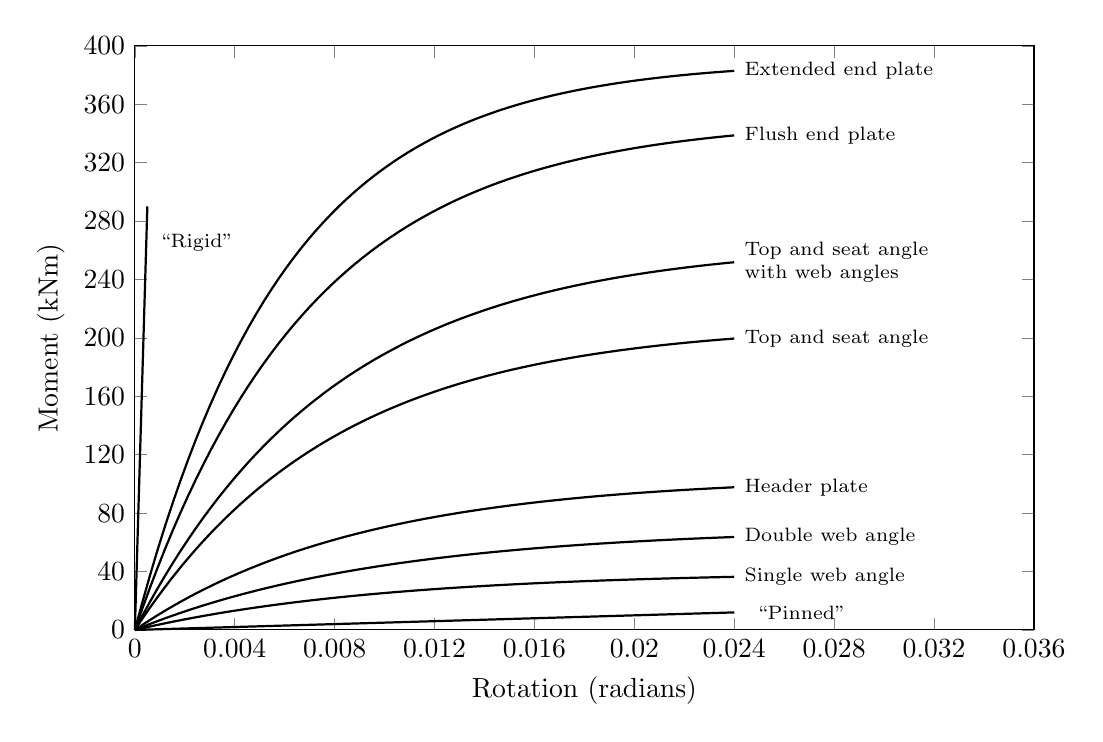
\begin{tikzpicture}
  \begin{axis}[
    width=13cm,height=9cm,
    xlabel={Rotation (radians)},ylabel={Moment (kNm)},
    xmin=0,xmax=0.036,ymin=0,ymax=400,
    xtick={0,0.004,...,0.036},xticklabel style={/pgf/number format/fixed,/pgf/number format/precision=3},
    ytick={0,40,...,400},
    clip=false,samples=80,domain=0:0.024,
    every axis plot/.append style={thick,black},
    cycle list={{black},{black},{black},{black},{black},{black},{black}},
    scaled x ticks=false,
  ]
    % curves of the form M = M0 * (1 - exp(-x/c))
    \addplot {390*(1-exp(-x/0.006))} node[right,font=\scriptsize] {Extended end plate};
    \addplot {350*(1-exp(-x/0.007))} node[right,font=\scriptsize] {Flush end plate};
    \addplot {265*(1-exp(-x/0.008))} node[right,align=left,font=\scriptsize] {Top and seat angle\\with web angles};
    \addplot {210*(1-exp(-x/0.008))} node[right,font=\scriptsize] {Top and seat angle};
    \addplot {105*(1-exp(-x/0.009))} node[right,font=\scriptsize] {Header plate};
    \addplot {70*(1-exp(-x/0.010))} node[right,font=\scriptsize] {Double web angle};
    \addplot {40*(1-exp(-x/0.010))} node[right,font=\scriptsize] {Single web angle};
    \draw[thick] (axis cs:0,0) -- (axis cs:0.0005,290); \node[right,font=\scriptsize] at (axis cs:0.0006,265) {``Rigid''};
    \draw[thick] (axis cs:0,0) -- (axis cs:0.024,12); \node[right,font=\scriptsize] at (axis cs:0.0245,12) {``Pinned''};
  \end{axis}
\end{tikzpicture}

  \caption{Typical moment-rotation curves (after Chen and Toma, 1994, Fig.~1.8).}
\end{figure}
In particular, three prediction equations were discussed in detail. The first was the analytical polynomial equation proposed by Frye and Morris (1976). The second was a curve-fitting equation using a modified exponential model proposed by Kishi and Chen (1986). The third model utilizes a three-parameter power model proposed by Kishi and Chen (1990), which is a simplified analytical model suitable for use in the analysis and design of steel frames.

The Kishi and Chen connection data base is made available to the reader in Chapter~3 of Chen and Toma. This data base includes connection types with semi-rigid moment-rotation characteristics similar to those reported in Goverdhan's data bank. Available test data on steel beam-to-column connections and comparison between experiment and theoretical results calculated using the three prediction models are available there.

\section{Symmetry and anti-symmetry}
The loads can be separated into two parts, one is the symmetric one, and the other is the anti-symmetric one. The DOFs for these two problems are listed in the table below.
\begin{center}
  \begin{tabular}{|c|c|c|}\hline
    & symmetric part & anti-symmetric part\\\hline
    DOFs & $u_b, v_b, \theta_b, v_c$ & $u_b, v_b, \theta_b, u_c, \theta_c$\\\hline
  \end{tabular}
\end{center}
\begin{fig}
  % Gable frame: loads, symmetric part, anti-symmetric part, and the half models
\begin{tikzpicture}[scale=0.62,font=\small]
  \newcommand{\gable}{\draw[thinmember] (0,0) -- (0,3) -- (2.5,4.2) -- (5,3) -- (5,0); \pic at (0,0) {fixed}; \pic at (5,0) {fixed};
    \node[left] at (0,0.3) {a}; \node[left] at (0,2.8) {b}; \node[above right] at (2.5,4.2) {c}; \node[right] at (5,2.8) {d}; \node[right] at (5,0.3) {e};}
  \newcommand{\halfgable}{\draw[thinmember] (0,0) -- (0,3) -- (2.5,4.2); \pic at (0,0) {fixed};
    \node[left] at (0,0.3) {a}; \node[left] at (0,2.8) {b};}
  % ---- original loading ----
  \begin{scope}[xshift=13cm,yshift=1cm]
    \gable
    \draw[load] (-1.5,3) -- (-0.1,3) node[pos=0,above] {8};
    \draw[load] (1.25,5.2) -- (1.25,3.7) node[pos=0,above] {12};
    \draw[load] (2.5,5.8) -- (2.5,4.3) node[pos=0,above] {10};
  \end{scope}
  % ---- symmetric ----
  \begin{scope}[yshift=-7cm]
    \gable
    \draw[load] (-1.5,3) -- (-0.1,3) node[pos=0,above] {4}; \draw[load] (6.5,3) -- (5.1,3) node[pos=0,above] {4};
    \draw[load] (1.25,5.2) -- (1.25,3.7) node[pos=0,above] {6}; \draw[load] (3.75,5.2) -- (3.75,3.7) node[pos=0,above] {6};
    \draw[load] (2.5,5.8) -- (2.5,4.3) node[pos=0,above] {5+5};
    \node[below] at (2.5,-0.6) {symmetric};
    \node at (7.5,2) {$\Longrightarrow$};
    \begin{scope}[xshift=9cm]
      \halfgable
      \draw[load] (-1.5,3) -- (-0.1,3) node[pos=0,above] {4};
      \draw[load] (1.25,5.2) -- (1.25,3.7) node[pos=0,above] {6};
      \draw[load] (2.5,5.8) -- (2.5,4.3) node[pos=0,above] {5};
      \node[below right] at (2.5,4.1) {c};
      \pic[rotate=-90] at (2.5,4.2) {roller}; \fill[hatch] (3.1,3.5) rectangle (3.3,4.9); \draw (3.1,3.5) -- (3.1,4.9);
    \end{scope}
  \end{scope}
  % ---- anti-symmetric ----
  \begin{scope}[yshift=-15cm]
    \gable
    \draw[load] (-1.5,3) -- (-0.1,3) node[pos=0,above] {4}; \draw[load] (5.1,3) -- (6.5,3) node[above] {4};
    \draw[load] (1.25,5.2) -- (1.25,3.7) node[pos=0,above] {6}; \draw[load] (3.75,3.7) -- (3.75,5.2) node[above] {6};
    \draw[load] (2.35,5.8) -- (2.35,4.3); \draw[load] (2.65,4.3) -- (2.65,5.8); \node[above] at (2.5,5.8) {5\ \,5};
    \node[below] at (2.5,-0.6) {anti-symmetric};
    \node at (7.5,2) {$\Longrightarrow$};
    \begin{scope}[xshift=9cm]
      \halfgable
      \draw[load] (-1.5,3) -- (-0.1,3) node[pos=0,above] {4};
      \draw[load] (1.25,5.2) -- (1.25,3.7) node[pos=0,above] {6};
      \node[above right] at (2.5,4.2) {c};
      \pic[rotate=-90] at (2.5,4.2) {roller}; % roller allowing horizontal movement, v_c = 0
    \end{scope}
  \end{scope}
\end{tikzpicture}

\end{fig}
\begin{center}
  \renewcommand{\arraystretch}{1.2}
  \begin{tabular}{|c|c|c|}\hline
    \multirow{6}{*}{The other DOFs} & \multirow{6}{*}{Sym.\ $\begin{aligned}u_d &= -u_b\\ v_d &= v_b\\ \theta_d &= -\theta_b\\ u_c &= 0\\ \theta_c &= 0\\ M_c &\neq 0\end{aligned}$}
    & \multirow{6}{*}{Anti-sym.\ $\begin{aligned}u_d &= u_b\\ v_d &= -v_b\\ \theta_d &= \theta_b\\ v_c &= 0\\ u_c &\neq 0\\ M_c &= 0\end{aligned}$}\\
    &&\\ &&\\ &&\\ &&\\ &&\\\hline
  \end{tabular}
\end{center}

\section{Effect of axial deformation (portal frame)}
\label{sec:axial-portal}
\begin{fig}
  % Portal frame with six DOFs (axial deformation included)
\begin{tikzpicture}[scale=0.9,font=\small]
  \draw[member] (0,0) -- (0,4) -- (4,4) -- (4,0);
  \pic at (0,0) {fixed}; \pic at (4,0) {fixed};
  \node at (2,2) {$EA, I, L$};
  \draw[load] (-1.6,4) -- (-0.9,4) node[pos=0,below] {$P$};
  \draw[load] (-0.8,4) -- (-0.1,4) node[pos=0,below] {$u_1$};
  \draw[load] (0,4.1) -- (0,5.0) node[above] {$u_2$};
  \draw[->,thick] (0.5,4.4) arc (30:170:0.5); \node[above left] at (-0.1,4.5) {$u_3$};
  \draw[load] (4.1,4) -- (5.0,4) node[right] {$u_4$};
  \draw[load] (4,4.1) -- (4,5.0) node[above] {$u_5$};
  \draw[->,thick] (4.5,4.4) arc (30:170:0.5); \node[above left] at (3.9,4.5) {$u_6$};
\end{tikzpicture}

\end{fig}
{\small
\begin{equation*}
  \Kmat = \begin{bmatrix}
    12E\frac{I}{L^3} + E\frac AL & 0 & 6E\frac{I}{L^2} & -E\frac AL & 0 & 0\\[3pt]
    0 & 12E\frac{I}{L^3} + E\frac AL & 6E\frac{I}{L^2} & 0 & -12E\frac{I}{L^3} & 6E\frac{I}{L^2}\\[3pt]
    6E\frac{I}{L^2} & 6E\frac{I}{L^2} & 8E\frac IL & 0 & -6E\frac{I}{L^2} & 2E\frac IL\\[3pt]
    -E\frac AL & 0 & 0 & 12E\frac{I}{L^3} + E\frac AL & 0 & 6E\frac{I}{L^2}\\[3pt]
    0 & -12E\frac{I}{L^3} & -6E\frac{I}{L^2} & 0 & 12E\frac{I}{L^3} + E\frac AL & -6E\frac{I}{L^2}\\[3pt]
    0 & 6E\frac{I}{L^2} & 2E\frac IL & 6E\frac{I}{L^2} & -6E\frac{I}{L^2} & 8E\frac IL
  \end{bmatrix},\qquad
  \Pvec = \Bmat{P\\ 0\\ 0\\ 0\\ 0\\ 0}
\end{equation*}
\begin{equation*}
  \bs{\Delta} = \Kmat^{-1}\Pvec = \Bmat{
    \frac{1}{12EI}L^3\frac{216I^2 + 84IAL^2 + 5A^2L^4}{72I^2 + 45IAL^2 + 7A^2L^4}P\\[4pt]
    3\frac{L^3}{(24I + 7AL^2)E}P\\[4pt]
    -\frac{1}{4EI}L^2\frac{96I^2 + 34IAL^2 + A^2L^4}{72I^2 + 45IAL^2 + 7A^2L^4}P\\[4pt]
    \frac{1}{12EI}L^3\frac{72I^2 + 42IAL^2 + 5A^2L^4}{72I^2 + 45IAL^2 + 7A^2L^4}P\\[4pt]
    -3\frac{L^3}{(24I + 7AL^2)E}P\\[4pt]
    -\frac{1}{4EI}L^2\frac{48I^2 + A^2L^4 + 20IAL^2}{72I^2 + 45IAL^2 + 7A^2L^4}P}
  = \Bmat{\frac{5}{84}\frac{PL^3}{EI}\\[4pt] 0\\[4pt] -\frac{1}{28}\frac{PL^2}{EI}\\[4pt] \frac{5}{84}\frac{PL^3}{EI}\\[4pt] 0\\[4pt] -\frac{1}{28}\frac{PL^2}{EI}}
  \quad\text{when }\frac{I}{AL^2}\to 0
\end{equation*}}
\begin{minipage}{0.4\linewidth}
\begin{align*}
  E &= 1.0\\ A &= 40(40)\ \mathrm{cm^2}\\ I &= \tfrac{1}{12}(40)^4\ \mathrm{cm^4}\\ L &= 300\ \mathrm{cm}
\end{align*}
\end{minipage}
\begin{minipage}{0.5\linewidth}\centering
\begin{tikzpicture}[scale=0.8]
  \fill[hatch] (0,0) rectangle (1.2,1.2); \draw (0,0) rectangle (1.2,1.2);
  \node[above] at (0.6,1.2) {40 cm}; \node[right] at (1.2,0.6) {40 cm};
\end{tikzpicture}
\end{minipage}
{\small
\begin{equation*}
  \begin{array}{cccc}
    A & 0.1A & 10A & 1000A\\[4pt]
    \Bmat{7.6487P\\ 7.9951\times10^{-2}P\\ -1.5679\times10^{-2}P\\ 7.5553P\\ -7.9951\times10^{-2}P\\ -1.5368\times10^{-2}P} &
    \Bmat{8.6378P\\ .76473P\\ -2.0933\times10^{-2}P\\ 7.7402P\\ -.76473P\\ -1.7941\times10^{-2}P} &
    \Bmat{7.5451P\\ 8.0316\times10^{-3}P\\ -1.5128\times10^{-2}P\\ 7.5357P\\ -8.0316\times10^{-3}P\\ -1.5097\times10^{-2}P} &
    \Bmat{7.5336P\\ 8.0357\times10^{-5}P\\ -1.5068\times10^{-2}P\\ 7.5335P\\ -8.0357\times10^{-5}P\\ -1.5067\times10^{-2}P}
  \end{array}
\end{equation*}}

\topic{Neglecting axial deformation ($u_2 = 0$, $u_5 = 0$; $u_1 = u_4$):}
\begin{equation*}
  \Kmat' = \begin{bmatrix}
    12E\frac{I}{L^3} + E\frac AL & 6E\frac{I}{L^2} & -E\frac AL & 0\\[3pt]
    6E\frac{I}{L^2} & 8E\frac IL & 0 & 2E\frac IL\\[3pt]
    -E\frac AL & 0 & 12E\frac{I}{L^3} + E\frac AL & 6E\frac{I}{L^2}\\[3pt]
    0 & 2E\frac IL & 6E\frac{I}{L^2} & 8E\frac IL
  \end{bmatrix}\quad\text{(DOFs } u_1, u_3, u_4, u_6\text{)}
\end{equation*}
\begin{equation*}
  \bs{\Delta}' = \Bmat{u_1\\ u_3\\ u_4\\ u_6} = \bmat{1 & 0 & 0\\ 0 & 1 & 0\\ 1 & 0 & 0\\ 0 & 0 & 1}\Bmat{u_1\\ u_3\\ u_6} = \Tmat\bs{\Delta}
\end{equation*}
\begin{equation*}
  \Kmat = \Tmat^\tr\Kmat'\Tmat = \bmat{1 & 0 & 1 & 0\\ 0 & 1 & 0 & 0\\ 0 & 0 & 0 & 1}
  \begin{bmatrix}
    12E\frac{I}{L^3} + E\frac AL & 6E\frac{I}{L^2} & -E\frac AL & 0\\[3pt]
    6E\frac{I}{L^2} & 8E\frac IL & 0 & 2E\frac IL\\[3pt]
    -E\frac AL & 0 & 12E\frac{I}{L^3} + E\frac AL & 6E\frac{I}{L^2}\\[3pt]
    0 & 2E\frac IL & 6E\frac{I}{L^2} & 8E\frac IL
  \end{bmatrix}\bmat{1 & 0 & 0\\ 0 & 1 & 0\\ 1 & 0 & 0\\ 0 & 0 & 1}
\end{equation*}
\begin{equation*}
  \therefore\Kmat = \bmat{24E\frac{I}{L^3} & 6E\frac{I}{L^2} & 6E\frac{I}{L^2}\\[3pt] 6E\frac{I}{L^2} & 8E\frac IL & 2E\frac IL\\[3pt] 6E\frac{I}{L^2} & 2E\frac IL & 8E\frac IL}
  \Rightarrow \Kmat^{-1} = \bmat{\frac{5}{84EI}L^3 & -\frac{1}{28EI}L^2 & -\frac{1}{28EI}L^2\\[3pt] -\frac{1}{28EI}L^2 & \frac{13}{84EI}L & -\frac{1}{84EI}L\\[3pt] -\frac{1}{28EI}L^2 & -\frac{1}{84EI}L & \frac{13}{84EI}L}
\end{equation*}
$\Pvec = \Tmat^\tr\Pvec'$, where $\Pvec'^\tr = \langle P, 0, 0, 0\rangle$
\begin{equation*}
  \bs{\Delta} = \Bmat{u_1\\ u_3\\ u_6} = \bmat{\frac{5}{84EI}L^3 & -\frac{1}{28EI}L^2 & -\frac{1}{28EI}L^2\\[3pt] -\frac{1}{28EI}L^2 & \frac{13}{84EI}L & -\frac{1}{84EI}L\\[3pt] -\frac{1}{28EI}L^2 & -\frac{1}{84EI}L & \frac{13}{84EI}L}\Bmat{P\\ 0\\ 0} = \Bmat{\frac{5}{84EI}PL^3\\[3pt] -\frac{1}{28EI}PL^2\\[3pt] -\frac{1}{28EI}PL^2}
\end{equation*}
With $E = 1.0$, $A = 40(40)$~cm$^2$, $I = \frac{1}{12}(40)^4$~cm$^4$, $L = 300$~cm:
\begin{equation*}
  \bs{\Delta} = \Bmat{\frac{3375}{448}P\\[3pt] -\frac{27}{1792}P\\[3pt] -\frac{27}{1792}P} = \Bmat{7.5335P\\ -1.5067\times10^{-2}P\\ -1.5067\times10^{-2}P}
\end{equation*}
\begin{center}
\begin{minipage}{0.4\linewidth}\centering% Portal frame with three DOFs (axial deformation neglected)
\begin{tikzpicture}[scale=0.9,font=\small]
  \draw[member] (0,0) -- (0,4) -- (4,4) -- (4,0);
  \pic at (0,0) {fixed}; \pic at (4,0) {fixed};
  \node at (2,2) {$EI, L$};
  \node[circle,draw,inner sep=1pt,fill=white] at (0,2) {\scriptsize 1};
  \node[circle,draw,inner sep=1pt,fill=white] at (2,4) {\scriptsize 2};
  \node[circle,draw,inner sep=1pt,fill=white] at (4,2) {\scriptsize 3};
  \draw[load] (-1.4,4) -- (-0.1,4) node[pos=0,left] {$v$};
  \draw[->,thick] (0.5,4.4) arc (30:170:0.5); \node[above left] at (-0.1,4.5) {$\theta_1$};
  \draw[->,thick] (4.5,4.4) arc (30:170:0.5); \node[above left] at (3.9,4.5) {$\theta_2$};
\end{tikzpicture}
\end{minipage}\hfill
\begin{minipage}{0.55\linewidth}
\begin{equation*}
  \Kmat = \begin{bmatrix}
    \dfrac{12EI}{L^3} + \dfrac{12EI}{L^3} & \dfrac{6EI}{L^2} & \dfrac{6EI}{L^2}\\[8pt]
    \dfrac{6EI}{L^2} & \dfrac{4EI}{L} + \dfrac{4EI}{L} & \dfrac{2EI}{L}\\[8pt]
    \dfrac{6EI}{L^2} & \dfrac{2EI}{L} & \dfrac{4EI}{L} + \dfrac{4EI}{L}
  \end{bmatrix}
\end{equation*}
\end{minipage}
\end{center}

\section{Beam elements in a rectangular frame with neglect of axial deformation}
No vertical displacements at both ends if the axial deformation of columns are very small and can be neglected.
\begin{center}
  \renewcommand{\arraystretch}{1.3}
  \begin{tabular}{|p{0.22\linewidth}|c|c|}\hline
    B1 & \begin{tikzpicture}[scale=0.7,font=\small,baseline=(current bounding box.center)]
  \draw[thinmember] (0,0) -- (5,0);
  \draw[->,thick] (0.6,0.45) arc (30:170:0.5); \node[above] at (0.1,0.7) {$\theta_1$};
  \draw[->,thick] (5.0,0.45) arc (30:170:0.5); \node[above] at (4.5,0.7) {$\theta_2$};
\end{tikzpicture}
 & $[k] = \dfrac{2EI}{L}\bmat{2 & 1\\ 1 & 2}$\\\hline
    B2\newline Pin at node 1\newline ($\theta_1$ is condensed) & \begin{tikzpicture}[scale=0.7,font=\small,baseline=(current bounding box.center)]
  \draw[thinmember] (0,0) -- (5,0); \node[node dot] at (0,0) {};
  \draw[->,thick] (5.0,0.45) arc (30:170:0.5); \node[above] at (4.5,0.7) {$\theta_2$};
\end{tikzpicture}
 & $k = \dfrac{3EI}{L}$\\\hline
    B3\newline Pin at node 2\newline ($\theta_2$ is condensed) & \begin{tikzpicture}[scale=0.7,font=\small,baseline=(current bounding box.center)]
  \draw[thinmember] (0,0) -- (5,0); \node[node dot] at (5,0) {};
  \draw[->,thick] (0.6,0.45) arc (30:170:0.5); \node[above] at (0.1,0.7) {$\theta_1$};
\end{tikzpicture}
 & $k = \dfrac{3EI}{L}$\\\hline
  \end{tabular}
\end{center}

\section{Column elements in a rectangular frame with neglect of axial deformation}
\begin{center}
  \renewcommand{\arraystretch}{1.3}
  \begin{tabular}{|c|c|c|}\hline
    C1 & \begin{tikzpicture}[scale=0.7,font=\small,baseline=(current bounding box.center)]
  \draw[thinmember] (0,0) -- (0,4);
  \draw[load] (0.1,4) -- (1.1,4) node[right] {$u_2$}; \draw[->,thick] (0.5,4.4) arc (30:170:0.5); \node[left] at (-0.4,4.5) {$\theta_2$};
  \draw[load] (0.1,0) -- (1.1,0) node[right] {$u_1$}; \draw[->,thick] (0.5,0.4) arc (30:170:0.5); \node[left] at (-0.4,0.5) {$\theta_1$};
\end{tikzpicture}
 &
      $[k] = \begin{array}{c}\begin{array}{cccc}\ \ u_1\ \ & \ \ \theta_1\ \ & \ \ u_2\ \ & \ \ \theta_2\ \ \end{array}\\
      \left[\begin{array}{cccc} 12EI/L^3 & -6EI/L^2 & -12EI/L^3 & -6EI/L^2\\ -6EI/L^2 & 4EI/L & 6EI/L^2 & 2EI/L\\ -12EI/L^3 & 6EI/L^2 & 12EI/L^3 & 6EI/L^2\\ -6EI/L^2 & 2EI/L & 6EI/L^2 & 4EI/L\end{array}\right]\end{array}$\\\hline
    C2 & \begin{tikzpicture}[scale=0.7,font=\small,baseline=(current bounding box.center)]
  \draw[thinmember] (0,0) -- (0,4); \node[node dot] at (0,4) {};
  \draw[load] (0.15,4) -- (1.1,4) node[right] {$u_2$};
  \draw[load] (0.1,0) -- (1.1,0) node[right] {$u_1$}; \draw[->,thick] (0.5,0.4) arc (30:170:0.5); \node[left] at (-0.4,0.5) {$\theta_1$};
\end{tikzpicture}
 &
      $[k] = \begin{array}{c}\begin{array}{ccc}\ \ u_1\ \ & \ \ \theta_1\ \ & \ \ u_2\ \ \end{array}\\
      \left[\begin{array}{ccc} 3EI/L^3 & -3EI/L^2 & -3EI/L^3\\ -3EI/L^2 & 3EI/L & 3EI/L^2\\ -3EI/L^3 & 3EI/L^2 & 3EI/L^3\end{array}\right]\end{array}$\\\hline
    C3 & \begin{tikzpicture}[scale=0.7,font=\small,baseline=(current bounding box.center)]
  \draw[thinmember] (0,0) -- (0,4); \node[node dot] at (0,0) {};
  \draw[load] (0.1,4) -- (1.1,4) node[right] {$u_2$}; \draw[->,thick] (0.5,4.4) arc (30:170:0.5); \node[left] at (-0.4,4.5) {$\theta_2$};
  \draw[load] (0.15,0) -- (1.1,0) node[right] {$u_1$};
\end{tikzpicture}
 &
      $[k] = \begin{array}{c}\begin{array}{ccc}\ \ u_1\ \ & \ \ u_2\ \ & \ \ \theta_2\ \ \end{array}\\
      \left[\begin{array}{ccc} 3EI/L^3 & -3EI/L^3 & -3EI/L^2\\ -3EI/L^3 & 3EI/L^3 & 3EI/L^2\\ -3EI/L^2 & 3EI/L^2 & 3EI/L\end{array}\right]\end{array}$\\\hline
  \end{tabular}
\end{center}

\begin{example}
\leavevmode
\begin{fig}
  %% Frame decomposition: whole frame = column 1 + beam 2 + column 3
\begin{tikzpicture}[scale=0.62,font=\small]
  \begin{scope}
    \draw[member] (0,0) -- (0,4) -- (4,4) -- (4,0); \pic at (0,0) {fixed}; \pic at (4,0) {fixed};
    \node[circle,draw,fill=white,inner sep=1pt,font=\scriptsize] at (0,2) {1}; \node[circle,draw,fill=white,inner sep=1pt,font=\scriptsize] at (2,4) {2}; \node[circle,draw,fill=white,inner sep=1pt,font=\scriptsize] at (4,2) {3};
    \draw[load] (4.1,4) -- (5.3,4) node[right] {$u_1$};
    \draw[->,thick] (0.45,4.35) arc (30:170:0.45); \node[above left,inner sep=1pt] at (-0.1,4.4) {$\theta_1$};
    \draw[->,thick] (4.45,4.35) arc (30:170:0.45); \node[above left,inner sep=1pt] at (3.9,4.4) {$\theta_2$};
  \end{scope}
  \node at (6.6,2) {\large $=$};
  \begin{scope}[xshift=8cm]
    \draw[member] (0,0) -- (0,4); \pic at (0,0) {fixed}; \node[circle,draw,fill=white,inner sep=1pt,font=\scriptsize] at (0,2) {1};
    \draw[load] (0.1,4) -- (1.3,4) node[right] {$u_1$};
    \draw[->,thick] (0.45,4.35) arc (30:170:0.45); \node[above left,inner sep=1pt] at (-0.1,4.4) {$\theta_1$};
    \node[below] at (0,-0.9) {C1};
  \end{scope}
  \node at (10,2) {\large $+$};
  \begin{scope}[xshift=11.5cm]
    \draw[member] (0,4) -- (4,4); \node[circle,draw,fill=white,inner sep=1pt,font=\scriptsize] at (2,4) {2};
    \draw[->,thick] (0.45,4.35) arc (30:170:0.45); \node[above left,inner sep=1pt] at (-0.1,4.4) {$\theta_1$};
    \draw[->,thick] (4.45,4.35) arc (30:170:0.45); \node[above left,inner sep=1pt] at (3.9,4.4) {$\theta_2$};
    \node[below] at (2,-0.9) {B1};
  \end{scope}
  \node at (17,2) {\large $+$};
  \begin{scope}[xshift=18.5cm]
    \draw[member] (0,0) -- (0,4); \node[circle,draw,fill=white,inner sep=1pt,font=\scriptsize] at (0,2) {3};
    \draw[load] (0.1,4) -- (1.3,4) node[right] {$u_1$};
    \draw[->,thick] (0.45,4.35) arc (30:170:0.45); \node[above left,inner sep=1pt] at (-0.1,4.4) {$\theta_2$};
    \node[below] at (0,-0.9) {C1};
  \end{scope}
\end{tikzpicture}

\end{fig}
{\small
\begin{align*}
  [k] &= \begin{array}{c}\begin{array}{ccc}\ u_1\ & \ \theta_1\ & \ \theta_2\ \end{array}\\ \left[\begin{array}{ccc}12EI/L^3 & 6EI/L^2 & 0\\ 6EI/L^2 & 4EI/L & 0\\ 0 & 0 & 0\end{array}\right]\end{array}
  + \begin{array}{c}\begin{array}{ccc}\ u_1\ & \ \theta_1\ & \ \theta_2\ \end{array}\\ \left[\begin{array}{ccc}0 & 0 & 0\\ 0 & 4EI/L & 2EI/L\\ 0 & 2EI/L & 4EI/L\end{array}\right]\end{array}
  + \begin{array}{c}\begin{array}{ccc}\ u_1\ & \ \theta_1\ & \ \theta_2\ \end{array}\\ \left[\begin{array}{ccc}12EI/L^3 & 0 & 6EI/L^2\\ 0 & 0 & 0\\ 6EI/L^2 & 0 & 4EI/L\end{array}\right]\end{array}\\
  &= \begin{array}{c}\begin{array}{ccc}\ u_1\ & \ \theta_1\ & \ \theta_2\ \end{array}\\ \left[\begin{array}{ccc}24EI/L^3 & 6EI/L^2 & 6EI/L^2\\ 6EI/L^2 & 8EI/L & 2EI/L\\ 6EI/L^2 & 2EI/L & 8EI/L\end{array}\right]\end{array}\qquad\text{(same as that given in the previous section)}
\end{align*}}
\end{example}

\begin{example}[Treatment of the internal hinge is the same as that given in Sec.~\ref{sec:end-hinge}]
\leavevmode

\textbf{Case 1:}
\begin{fig}
  %% Frame decomposition: whole frame = column 1 + beam 2 + column 3
\begin{tikzpicture}[scale=0.62,font=\small]
  \begin{scope}
    \draw[member] (0,0) -- (0,4) -- (4,4) -- (4,0); \pic at (0,0) {fixed}; \pic at (4,0) {fixed};
    \node[circle,draw,fill=white,inner sep=1pt,font=\scriptsize] at (0,2) {1}; \node[circle,draw,fill=white,inner sep=1pt,font=\scriptsize] at (2,4) {2}; \node[circle,draw,fill=white,inner sep=1pt,font=\scriptsize] at (4,2) {3};
    \node[node dot] at (0,4) {};
    \draw[load] (4.1,4) -- (5.3,4) node[right] {$u_1$};
    \draw[->,thick] (0.45,4.35) arc (30:170:0.45); \node[above left,inner sep=1pt] at (-0.1,4.4) {$\theta_1$};
    \draw[->,thick] (4.45,4.35) arc (30:170:0.45); \node[above left,inner sep=1pt] at (3.9,4.4) {$\theta_2$};
  \end{scope}
  \node at (6.6,2) {\large $=$};
  \begin{scope}[xshift=8cm]
    \draw[member] (0,0) -- (0,4); \pic at (0,0) {fixed}; \node[circle,draw,fill=white,inner sep=1pt,font=\scriptsize] at (0,2) {1};
    \draw[load] (0.1,4) -- (1.3,4) node[right] {$u_1$};
    \draw[->,thick] (0.45,4.35) arc (30:170:0.45); \node[above left,inner sep=1pt] at (-0.1,4.4) {$\theta_1$};
    \node[below] at (0,-0.9) {C1};
  \end{scope}
  \node at (10,2) {\large $+$};
  \begin{scope}[xshift=11.5cm]
    \draw[member] (0,4) -- (4,4); \node[circle,draw,fill=white,inner sep=1pt,font=\scriptsize] at (2,4) {2};
    \node[node dot] at (0,4) {};
    \draw[->,thick] (4.45,4.35) arc (30:170:0.45); \node[above left,inner sep=1pt] at (3.9,4.4) {$\theta_2$};
    \node[below] at (2,-0.9) {B2};
  \end{scope}
  \node at (17,2) {\large $+$};
  \begin{scope}[xshift=18.5cm]
    \draw[member] (0,0) -- (0,4); \node[circle,draw,fill=white,inner sep=1pt,font=\scriptsize] at (0,2) {3};
    \draw[load] (0.1,4) -- (1.3,4) node[right] {$u_1$};
    \draw[->,thick] (0.45,4.35) arc (30:170:0.45); \node[above left,inner sep=1pt] at (-0.1,4.4) {$\theta_2$};
    \node[below] at (0,-0.9) {C1};
  \end{scope}
\end{tikzpicture}

\end{fig}
{\small
\begin{align*}
  [k] &= \begin{array}{c}\begin{array}{ccc}\ u_1\ & \ \theta_1\ & \ \theta_2\ \end{array}\\ \left[\begin{array}{ccc}12EI/L^3 & 6EI/L^2 & 0\\ 6EI/L^2 & 4EI/L & 0\\ 0 & 0 & 0\end{array}\right]\end{array}
  + \begin{array}{c}\begin{array}{ccc}u_1 & \theta_1 & \ \theta_2\ \end{array}\\ \left[\begin{array}{ccc}0 & 0 & 0\\ 0 & 0 & 0\\ 0 & 0 & 3EI/L\end{array}\right]\end{array}
  + \begin{array}{c}\begin{array}{ccc}\ u_1\ & \ \theta_1\ & \ \theta_2\ \end{array}\\ \left[\begin{array}{ccc}12EI/L^3 & 0 & 6EI/L^2\\ 0 & 0 & 0\\ 6EI/L^2 & 0 & 4EI/L\end{array}\right]\end{array}\\
  &= \begin{array}{c}\begin{array}{ccc}\ u_1\ & \ \theta_1\ & \ \theta_2\ \end{array}\\ \left[\begin{array}{ccc}24EI/L^3 & 6EI/L^2 & 6EI/L^2\\ 6EI/L^2 & 4EI/L & 0\\ 6EI/L^2 & 0 & 7EI/L\end{array}\right]\end{array}
\end{align*}}
\textbf{Case 2:}
\begin{fig}
  %% Frame decomposition: whole frame = column 1 + beam 2 + column 3
\begin{tikzpicture}[scale=0.62,font=\small]
  \begin{scope}
    \draw[member] (0,0) -- (0,4) -- (4,4) -- (4,0); \pic at (0,0) {fixed}; \pic at (4,0) {fixed};
    \node[circle,draw,fill=white,inner sep=1pt,font=\scriptsize] at (0,2) {1}; \node[circle,draw,fill=white,inner sep=1pt,font=\scriptsize] at (2,4) {2}; \node[circle,draw,fill=white,inner sep=1pt,font=\scriptsize] at (4,2) {3};
    \node[node dot] at (0,4) {};
    \draw[load] (4.1,4) -- (5.3,4) node[right] {$u_1$};
    \draw[->,thick] (4.45,4.35) arc (30:170:0.45); \node[above left,inner sep=1pt] at (3.9,4.4) {$\theta_2$};
    \draw[->,thick] (0.45,4.35) arc (30:170:0.45); \node[above right,inner sep=1pt] at (0.1,4.4) {$\theta_1$};
  \end{scope}
  \node at (6.6,2) {\large $=$};
  \begin{scope}[xshift=8cm]
    \draw[member] (0,0) -- (0,4); \pic at (0,0) {fixed}; \node[circle,draw,fill=white,inner sep=1pt,font=\scriptsize] at (0,2) {1};
    \node[node dot] at (0,4) {};
    \draw[load] (0.1,4) -- (1.3,4) node[right] {$u_1$};
    \node[below] at (0,-0.9) {C2};
  \end{scope}
  \node at (10,2) {\large $+$};
  \begin{scope}[xshift=11.5cm]
    \draw[member] (0,4) -- (4,4); \node[circle,draw,fill=white,inner sep=1pt,font=\scriptsize] at (2,4) {2};
    \draw[->,thick] (0.45,4.35) arc (30:170:0.45); \node[above left,inner sep=1pt] at (-0.1,4.4) {$\theta_1$};
    \draw[->,thick] (4.45,4.35) arc (30:170:0.45); \node[above left,inner sep=1pt] at (3.9,4.4) {$\theta_2$};
    \node[below] at (2,-0.9) {B1};
  \end{scope}
  \node at (17,2) {\large $+$};
  \begin{scope}[xshift=18.5cm]
    \draw[member] (0,0) -- (0,4); \node[circle,draw,fill=white,inner sep=1pt,font=\scriptsize] at (0,2) {3};
    \draw[load] (0.1,4) -- (1.3,4) node[right] {$u_1$};
    \draw[->,thick] (0.45,4.35) arc (30:170:0.45); \node[above left,inner sep=1pt] at (-0.1,4.4) {$\theta_2$};
    \node[below] at (0,-0.9) {C1};
  \end{scope}
\end{tikzpicture}

\end{fig}
{\small
\begin{align*}
  [k] &= \begin{array}{c}\begin{array}{ccc}\ u_1\ & \theta_1 & \theta_2\end{array}\\ \left[\begin{array}{ccc}3EI/L^3 & 0 & 0\\ 0 & 0 & 0\\ 0 & 0 & 0\end{array}\right]\end{array}
  + \begin{array}{c}\begin{array}{ccc}\ u_1\ & \ \theta_1\ & \ \theta_2\ \end{array}\\ \left[\begin{array}{ccc}0 & 0 & 0\\ 0 & 4EI/L & 2EI/L\\ 0 & 2EI/L & 4EI/L\end{array}\right]\end{array}
  + \begin{array}{c}\begin{array}{ccc}\ u_1\ & \ \theta_1\ & \ \theta_2\ \end{array}\\ \left[\begin{array}{ccc}12EI/L^3 & 0 & 6EI/L^2\\ 0 & 0 & 0\\ 6EI/L^2 & 0 & 4EI/L\end{array}\right]\end{array}\\
  &= \begin{array}{c}\begin{array}{ccc}\ u_1\ & \ \theta_1\ & \ \theta_2\ \end{array}\\ \left[\begin{array}{ccc}15EI/L^3 & 0 & 6EI/L^2\\ 0 & 4EI/L & 2EI/L\\ 6EI/L^2 & 2EI/L & 8EI/L\end{array}\right]\end{array}
\end{align*}}
\textbf{Case 3:}
\begin{fig}
  %% Frame decomposition: whole frame = column 1 + beam 2 + column 3
\begin{tikzpicture}[scale=0.62,font=\small]
  \begin{scope}
    \draw[member] (0,0) -- (0,4) -- (4,4) -- (4,0); \pic at (0,0) {fixed}; \pic at (4,0) {fixed};
    \node[circle,draw,fill=white,inner sep=1pt,font=\scriptsize] at (0,2) {1}; \node[circle,draw,fill=white,inner sep=1pt,font=\scriptsize] at (2,4) {2}; \node[circle,draw,fill=white,inner sep=1pt,font=\scriptsize] at (4,2) {3};
    \node[node dot] at (0,4) {};
    \draw[load] (4.1,4) -- (5.3,4) node[right] {$u_1$};
    \draw[->,thick] (4.45,4.35) arc (30:170:0.45); \node[above left,inner sep=1pt] at (3.9,4.4) {$\theta_2$};
  \end{scope}
  \node at (6.6,2) {\large $=$};
  \begin{scope}[xshift=8cm]
    \draw[member] (0,0) -- (0,4); \pic at (0,0) {fixed}; \node[circle,draw,fill=white,inner sep=1pt,font=\scriptsize] at (0,2) {1};
    \node[node dot] at (0,4) {};
    \draw[load] (0.1,4) -- (1.3,4) node[right] {$u_1$};
    \node[below] at (0,-0.9) {C2};
  \end{scope}
  \node at (10,2) {\large $+$};
  \begin{scope}[xshift=11.5cm]
    \draw[member] (0,4) -- (4,4); \node[circle,draw,fill=white,inner sep=1pt,font=\scriptsize] at (2,4) {2};
    \node[node dot] at (0,4) {};
    \draw[->,thick] (4.45,4.35) arc (30:170:0.45); \node[above left,inner sep=1pt] at (3.9,4.4) {$\theta_2$};
    \node[below] at (2,-0.9) {B2};
  \end{scope}
  \node at (17,2) {\large $+$};
  \begin{scope}[xshift=18.5cm]
    \draw[member] (0,0) -- (0,4); \node[circle,draw,fill=white,inner sep=1pt,font=\scriptsize] at (0,2) {3};
    \draw[load] (0.1,4) -- (1.3,4) node[right] {$u_1$};
    \draw[->,thick] (0.45,4.35) arc (30:170:0.45); \node[above left,inner sep=1pt] at (-0.1,4.4) {$\theta_2$};
    \node[below] at (0,-0.9) {C1};
  \end{scope}
\end{tikzpicture}

\end{fig}
{\small
\begin{align*}
  [k] &= \begin{array}{c}\begin{array}{cc}\ u_1\ & \theta_2\end{array}\\ \left[\begin{array}{cc}3EI/L^3 & 0\\ 0 & 0\end{array}\right]\end{array}
  + \begin{array}{c}\begin{array}{cc}u_1 & \ \theta_2\ \end{array}\\ \left[\begin{array}{cc}0 & 0\\ 0 & 3EI/L\end{array}\right]\end{array}
  + \begin{array}{c}\begin{array}{cc}\ u_1\ & \ \theta_2\ \end{array}\\ \left[\begin{array}{cc}12EI/L^3 & 6EI/L^2\\ 6EI/L^2 & 4EI/L\end{array}\right]\end{array}
  = \begin{array}{c}\begin{array}{cc}\ u_1\ & \ \theta_2\ \end{array}\\ \left[\begin{array}{cc}15EI/L^3 & 6EI/L^2\\ 6EI/L^2 & 7EI/L\end{array}\right]\end{array}
\end{align*}}
\textbf{Case 4:}
\begin{fig}
  %% Frame decomposition: whole frame = column 1 + beam 2 + column 3
\begin{tikzpicture}[scale=0.62,font=\small]
  \begin{scope}
    \draw[member] (0,0) -- (0,4) -- (4,4) -- (4,0); \pic at (0,0) {fixed}; \pic at (4,0) {fixed};
    \node[circle,draw,fill=white,inner sep=1pt,font=\scriptsize] at (0,2) {1}; \node[circle,draw,fill=white,inner sep=1pt,font=\scriptsize] at (2,4) {2}; \node[circle,draw,fill=white,inner sep=1pt,font=\scriptsize] at (4,2) {3};
    \node[node dot] at (0,4) {};
    \draw[load] (4.1,4) -- (5.3,4) node[right] {$u_1$};
    \draw[->,thick] (0.45,4.35) arc (30:170:0.45); \node[above left,inner sep=1pt] at (-0.1,4.4) {$\theta_{1l}$};
    \draw[->,thick] (4.45,4.35) arc (30:170:0.45); \node[above left,inner sep=1pt] at (3.9,4.4) {$\theta_2$};
    \draw[->,thick] (0.45,4.35) arc (30:170:0.45); \node[above right,inner sep=1pt] at (0.1,4.4) {$\theta_{1r}$};
  \end{scope}
  \node at (6.6,2) {\large $=$};
  \begin{scope}[xshift=8cm]
    \draw[member] (0,0) -- (0,4); \pic at (0,0) {fixed}; \node[circle,draw,fill=white,inner sep=1pt,font=\scriptsize] at (0,2) {1};
    \draw[load] (0.1,4) -- (1.3,4) node[right] {$u_1$};
    \draw[->,thick] (0.45,4.35) arc (30:170:0.45); \node[above left,inner sep=1pt] at (-0.1,4.4) {$\theta_{1l}$};
    \node[below] at (0,-0.9) {C1};
  \end{scope}
  \node at (10,2) {\large $+$};
  \begin{scope}[xshift=11.5cm]
    \draw[member] (0,4) -- (4,4); \node[circle,draw,fill=white,inner sep=1pt,font=\scriptsize] at (2,4) {2};
    \node[node dot] at (0,4) {};
    \draw[->,thick] (0.45,4.35) arc (30:170:0.45); \node[above left,inner sep=1pt] at (-0.1,4.4) {$\theta_{1r}$};
    \draw[->,thick] (4.45,4.35) arc (30:170:0.45); \node[above left,inner sep=1pt] at (3.9,4.4) {$\theta_2$};
    \node[below] at (2,-0.9) {B1};
  \end{scope}
  \node at (17,2) {\large $+$};
  \begin{scope}[xshift=18.5cm]
    \draw[member] (0,0) -- (0,4); \node[circle,draw,fill=white,inner sep=1pt,font=\scriptsize] at (0,2) {3};
    \draw[load] (0.1,4) -- (1.3,4) node[right] {$u_1$};
    \draw[->,thick] (0.45,4.35) arc (30:170:0.45); \node[above left,inner sep=1pt] at (-0.1,4.4) {$\theta_2$};
    \node[below] at (0,-0.9) {C1};
  \end{scope}
\end{tikzpicture}

\end{fig}
{\footnotesize\setlength{\arraycolsep}{3pt}
\begin{align*}
  [k] &= \begin{array}{c}\begin{array}{cccc}\ u_1\ & \ \theta_{1l}\ & \theta_{1r} & \theta_2\end{array}\\ \left[\begin{array}{cccc}12EI/L^3 & 6EI/L^2 & 0 & 0\\ 6EI/L^2 & 4EI/L & 0 & 0\\ 0 & 0 & 0 & 0\\ 0 & 0 & 0 & 0\end{array}\right]\end{array}
  + \begin{array}{c}\begin{array}{cccc}u_1 & \theta_{1l} & \ \theta_{1r}\ & \ \theta_2\ \end{array}\\ \left[\begin{array}{cccc}0 & 0 & 0 & 0\\ 0 & 0 & 0 & 0\\ 0 & 0 & 4EI/L & 2EI/L\\ 0 & 0 & 2EI/L & 4EI/L\end{array}\right]\end{array}
  + \begin{array}{c}\begin{array}{cccc}\ u_1\ & \theta_{1l} & \theta_{1r} & \ \theta_2\ \end{array}\\ \left[\begin{array}{cccc}12EI/L^3 & 0 & 0 & 6EI/L^2\\ 0 & 0 & 0 & 0\\ 0 & 0 & 0 & 0\\ 6EI/L^2 & 0 & 0 & 4EI/L\end{array}\right]\end{array}\\
  &= \begin{array}{c}\begin{array}{cccc}\ u_1\ & \ \theta_{1l}\ & \ \theta_{1r}\ & \ \theta_2\ \end{array}\\ \left[\begin{array}{cccc}24EI/L^3 & 6EI/L^2 & 0 & 6EI/L^2\\ 6EI/L^2 & 4EI/L & 0 & 0\\ 0 & 0 & 4EI/L & 2EI/L\\ 6EI/L^2 & 0 & 2EI/L & 8EI/L\end{array}\right]\end{array}
\end{align*}}
Discussion: To reduce the number of DOFs, condensed elements are usually used for both beams and columns, i.e.\ case 3.
\end{example}

\begin{example}[Note that the column is continuous at node B]
\leavevmode

\begin{minipage}{0.55\linewidth}\centering% Example 3: two-storey frame with hinges at A and B (column continuous at B)
\begin{tikzpicture}[scale=0.85,font=\small]
  \draw[member] (0,0) -- (0,5) -- (3.5,5) -- (3.5,0); \draw[member] (0,2.5) -- (6,2.5) -- (6,0);
  \pic at (0,0) {pin}; \pic at (3.5,0) {fixed}; \pic at (6,0) {fixed};
  \node[node dot] at (3.5,5) {}; \node[node dot] at (3.5,2.5) {};
  \node[above] at (3.5,5.1) {$A$}; \node[above right] at (3.55,2.55) {$B$};
  \newcommand{\mem}[2]{\node[circle,draw,fill=white,inner sep=1pt,font=\scriptsize] at #1 {#2};}
  \mem{(0,1.2)}{1} \mem{(3.5,1.2)}{2} \mem{(6,1.2)}{3} \mem{(0,3.8)}{4} \mem{(3.5,3.8)}{5}
  \mem{(1.75,2.5)}{6} \mem{(4.75,2.5)}{7} \mem{(1.75,5)}{8}
  \draw[load] (3.6,5) -- (4.8,5) node[right] {$u_2$};
  \draw[load] (6.1,2.5) -- (7.3,2.5) node[right] {$u_1$};
  \draw[->,thick] (0.5,5.35) arc (30:170:0.5); \node[left] at (-0.4,5.5) {$\theta_4$};
  \draw[->,thick] (0.5,2.85) arc (30:170:0.5); \node[left] at (-0.4,3.0) {$\theta_1$};
  \draw[->,thick] (3.3,2.85) arc (30:170:0.5); \node[left] at (2.4,3.0) {$\theta_2$};
  \draw[->,thick] (6.5,2.85) arc (30:170:0.5); \node[left] at (5.6,3.0) {$\theta_3$};
\end{tikzpicture}
\end{minipage}\hfill
\begin{minipage}{0.42\linewidth}
  \begin{tabular}{lll}
    \textbf{Element} & \textbf{Type} & \textbf{DOFs}\\
    1 & C3 & $u_1, \theta_1$\\
    2 & C1 & $u_1, \theta_2$\\
    3 & C1 & $u_1, \theta_3$\\
    4 & C1 & $u_1, \theta_1, u_2, \theta_4$\\
    5 & C2 & $u_1, \theta_2, u_2$\\
    6 & B1 & $\theta_1, \theta_2$\\
    7 & B2 & $\theta_3$\\
    8 & B3 & $\theta_4$
  \end{tabular}
\end{minipage}
\end{example}

\section{Equivalent forces for uniformly distributed loads and centre point load}
\begin{figure}[H]
  \centering
  % Equivalent forces for uniformly distributed loads and centre point load (B1-B3, C1-C3)
\begin{tikzpicture}[scale=0.72,font=\scriptsize]
  \newcommand{\udl}{\foreach \x in {0.3,0.8,...,4.8}{\draw[->] (\x,1.0) -- (\x,0.15);} \draw (0.3,1.0) -- (4.8,1.0);}
  \newcommand{\hudl}{\foreach \y in {0.3,0.8,...,3.8}{\draw[->] (-1.0,\y) -- (-0.15,\y);} \draw (-1.0,0.3) -- (-1.0,3.8);}
  % ================= beams =================
  % B1
  \begin{scope}
    \node[left] at (-0.5,0) {B1};
    \draw[thinmember] (0,0) -- (5,0); \udl
    \draw[->,thick] (0.6,-0.1) arc (30:170:0.5); \node[left] at (-0.2,-0.2) {$\frac{wL^2}{12}$};
    \draw[->,thick] (4.4,-0.4) arc (200:20:0.5); \node[right] at (5.2,-0.2) {$\frac{wL^2}{12}$};
  \end{scope}
  \begin{scope}[xshift=9cm]
    \draw[thinmember] (0,0) -- (5,0); \draw[load] (2.5,1.2) -- (2.5,0.15) node[pos=0,above] {$P$};
    \draw[->,thick] (0.6,-0.1) arc (30:170:0.5); \node[left] at (-0.2,-0.2) {$\frac{PL}{8}$};
    \draw[->,thick] (4.4,-0.4) arc (200:20:0.5); \node[right] at (5.2,-0.2) {$\frac{PL}{8}$};
  \end{scope}
  % B2
  \begin{scope}[yshift=-2.8cm]
    \node[left] at (-0.5,0) {B2};
    \draw[thinmember] (0,0) -- (5,0); \node[node dot] at (0,0) {}; \udl
    \draw[->,thick] (4.4,-0.4) arc (200:20:0.5); \node[right] at (5.2,-0.2) {$\frac{wL^2}{8}$};
  \end{scope}
  \begin{scope}[xshift=9cm,yshift=-2.8cm]
    \draw[thinmember] (0,0) -- (5,0); \node[node dot] at (0,0) {}; \draw[load] (2.5,1.2) -- (2.5,0.15) node[pos=0,above] {$P$};
    \draw[->,thick] (4.4,-0.4) arc (200:20:0.5); \node[right] at (5.2,-0.2) {$\frac{3PL}{16}$};
  \end{scope}
  % B3
  \begin{scope}[yshift=-5.6cm]
    \node[left] at (-0.5,0) {B3};
    \draw[thinmember] (0,0) -- (5,0); \node[node dot] at (5,0) {}; \udl
    \draw[->,thick] (0.6,-0.1) arc (30:170:0.5); \node[left] at (-0.2,-0.2) {$\frac{wL^2}{8}$};
  \end{scope}
  \begin{scope}[xshift=9cm,yshift=-5.6cm]
    \draw[thinmember] (0,0) -- (5,0); \node[node dot] at (5,0) {}; \draw[load] (2.5,1.2) -- (2.5,0.15) node[pos=0,above] {$P$};
    \draw[->,thick] (0.6,-0.1) arc (30:170:0.5); \node[left] at (-0.2,-0.2) {$\frac{3PL}{16}$};
  \end{scope}
  % ================= columns =================
  % C1
  \begin{scope}[yshift=-12.5cm]
    \node[left] at (-1.6,2) {C1};
    \draw[thinmember] (0,0) -- (0,4); \hudl
    \draw[load] (0.1,4) -- (1.0,4) node[right] {$\frac{wL}{2}$}; \draw[->,thick] (0.5,4.35) arc (30:170:0.45); \node[above right] at (0.5,4.4) {$\frac{wL^2}{12}$};
    \draw[load] (0.1,0) -- (1.0,0) node[right] {$\frac{wL}{2}$}; \draw[->,thick] (0.5,0.35) arc (30:170:0.45); \node[above right] at (0.5,0.4) {$\frac{wL^2}{12}$};
  \end{scope}
  \begin{scope}[xshift=9cm,yshift=-12.5cm]
    \draw[thinmember] (0,0) -- (0,4); \draw[load] (-1.2,2) -- (-0.15,2) node[pos=0,above] {$P$};
    \draw[load] (0.1,4) -- (1.0,4) node[right] {$\frac P2$}; \draw[->,thick] (0.5,4.35) arc (30:170:0.45); \node[above right] at (0.5,4.4) {$\frac{PL}{8}$};
    \draw[load] (0.1,0) -- (1.0,0) node[right] {$\frac P2$}; \draw[->,thick] (0.5,0.35) arc (30:170:0.45); \node[above right] at (0.5,0.4) {$\frac{PL}{8}$};
  \end{scope}
  % C2 (hinge at top)
  \begin{scope}[yshift=-18.5cm]
    \node[left] at (-1.6,2) {C2};
    \draw[thinmember] (0,0) -- (0,4); \node[node dot] at (0,4) {}; \hudl
    \draw[load] (0.15,4) -- (1.0,4) node[right] {$\frac38wL$};
    \draw[load] (0.1,0) -- (1.0,0) node[right] {$\frac58wL$}; \draw[->,thick] (0.5,0.35) arc (30:170:0.45); \node[above right] at (0.5,0.4) {$\frac{wL^2}{8}$};
  \end{scope}
  \begin{scope}[xshift=9cm,yshift=-18.5cm]
    \draw[thinmember] (0,0) -- (0,4); \node[node dot] at (0,4) {}; \draw[load] (-1.2,2) -- (-0.15,2) node[pos=0,above] {$P$};
    \draw[load] (0.15,4) -- (1.0,4) node[right] {$\frac{5}{16}P$};
    \draw[load] (0.1,0) -- (1.0,0) node[right] {$\frac{11}{16}P$}; \draw[->,thick] (0.5,0.35) arc (30:170:0.45); \node[above right] at (0.5,0.4) {$\frac{3}{16}PL$};
  \end{scope}
  % C3 (hinge at bottom)
  \begin{scope}[yshift=-24.5cm]
    \node[left] at (-1.6,2) {C3};
    \draw[thinmember] (0,0) -- (0,4); \node[node dot] at (0,0) {}; \hudl
    \draw[load] (0.1,4) -- (1.0,4) node[right] {$\frac58wL$}; \draw[->,thick] (0.5,4.35) arc (30:170:0.45); \node[above right] at (0.5,4.4) {$\frac{wL^2}{8}$};
    \draw[load] (0.15,0) -- (1.0,0) node[right] {$\frac38wL$};
  \end{scope}
  \begin{scope}[xshift=9cm,yshift=-24.5cm]
    \draw[thinmember] (0,0) -- (0,4); \node[node dot] at (0,0) {}; \draw[load] (-1.2,2) -- (-0.15,2) node[pos=0,above] {$P$};
    \draw[load] (0.1,4) -- (1.0,4) node[right] {$\frac{11}{16}P$}; \draw[->,thick] (0.5,4.35) arc (30:170:0.45); \node[above right] at (0.5,4.4) {$\frac{3}{16}PL$};
    \draw[load] (0.15,0) -- (1.0,0) node[right] {$\frac{5}{16}P$};
  \end{scope}
\end{tikzpicture}

\end{figure}

\begin{example}[Frame with a hinge at the top-left corner under three loadings]
\leavevmode
\begin{fig}
  % Example 2: the three loading cases on the frame with a hinge at the top-left corner
\begin{tikzpicture}[scale=0.6,font=\small]
  \newcommand{\hframe}{\draw[member] (0,0) -- (0,4) -- (4,4) -- (4,0); \pic at (0,0) {fixed}; \pic at (4,0) {fixed}; \node[node dot] at (0,4) {};}
  \begin{scope} \hframe \draw[load] (-1.4,4) -- (-0.15,4) node[pos=0,below] {$P$}; \end{scope}
  \begin{scope}[xshift=7cm] \hframe \draw[load] (-1.4,2) -- (-0.1,2) node[pos=0,below] {$P$}; \end{scope}
  \begin{scope}[xshift=14cm] \hframe \foreach \x in {0.3,0.8,...,3.8}{\draw[->] (\x,5.0) -- (\x,4.15);} \draw (0.3,5.0) -- (3.8,5.0); \node[above] at (2,5.0) {$w$}; \end{scope}
\end{tikzpicture}

\end{fig}
{\scriptsize
\renewcommand{\arraystretch}{1.0}
\begin{longtable}{|c|c|c|c|}\hline
  \textbf{Case} & Load 1 ($P$ at the corner) & Load 2 ($P$ at mid-height) & Load 3 ($w$ on the beam)\\\hline
  \shortstack{Case 1:\\[2pt] \begin{tikzpicture}[scale=0.5,font=\scriptsize,baseline=(current bounding box.center)]
  \draw[member] (0,0) -- (0,4) -- (4,4) -- (4,0); \pic at (0,0) {fixed}; \pic at (4,0) {fixed};
  \node[node dot] at (0,4) {};
  \draw[load] (4.1,4) -- (5.3,4) node[right] {$u_1$};
  \draw[->,thick] (4.45,4.35) arc (30:170:0.45); \node[above left,inner sep=1pt] at (3.9,4.4) {$\theta_2$};
  \draw[->,thick] (0.45,4.35) arc (30:170:0.45); \node[above left,inner sep=1pt] at (-0.1,4.4) {$\theta_1$};
\end{tikzpicture}
} &
  $\begin{aligned}\Pvec &= \Bmat{P\\ 0\\ 0}\\ \Bmat{u_1\\ \theta_1(\theta_{1l})\\ \theta_2} &= \Bmat{\frac{7}{69}\frac{PL^3}{EI}\\[2pt] -\frac{7}{46}\frac{PL^2}{EI}\\[2pt] -\frac{2}{23}\frac{PL^2}{EI}}\end{aligned}$ &
  $\begin{aligned}\Pvec &= \Bmat{\frac P2\\[2pt] \frac{PL}{8}\\[2pt] 0}\\ \Bmat{u_1\\ \theta_1(\theta_{1l})\\ \theta_2} &= \Bmat{\frac{35}{1104}\frac{PL^3}{EI}\\[2pt] -\frac{3}{184}\frac{PL^2}{EI}\\[2pt] -\frac{5}{184}\frac{PL^2}{EI}}\end{aligned}$ &
  $\begin{aligned}\Pvec &= \Bmat{0\\ 0\\ \frac{wL^2}{8}}\\ \Bmat{u_1\\ \theta_1(\theta_{1l})\\ \theta_2} &= \Bmat{-\frac{1}{92}\frac{wL^4}{EI}\\[2pt] \frac{3}{184}\frac{wL^3}{EI}\\[2pt] \frac{5}{184}\frac{wL^3}{EI}}\end{aligned}$\\\hline
  \shortstack{Case 2:\\[2pt] \begin{tikzpicture}[scale=0.5,font=\scriptsize,baseline=(current bounding box.center)]
  \draw[member] (0,0) -- (0,4) -- (4,4) -- (4,0); \pic at (0,0) {fixed}; \pic at (4,0) {fixed};
  \node[node dot] at (0,4) {};
  \draw[load] (4.1,4) -- (5.3,4) node[right] {$u_1$};
  \draw[->,thick] (4.45,4.35) arc (30:170:0.45); \node[above left,inner sep=1pt] at (3.9,4.4) {$\theta_2$};
  \draw[->,thick] (0.9,4.35) arc (30:170:0.45); \node[above right,inner sep=1pt] at (0.6,4.4) {$\theta_1$};
\end{tikzpicture}
} &
  $\begin{aligned}\Pvec &= \Bmat{P\\ 0\\ 0}\\ \Bmat{u_1\\ \theta_1(\theta_{1r})\\ \theta_2} &= \Bmat{\frac{7}{69}\frac{PL^3}{EI}\\[2pt] \frac{1}{23}\frac{PL^2}{EI}\\[2pt] -\frac{2}{23}\frac{PL^2}{EI}}\end{aligned}$ &
  $\begin{aligned}\Pvec &= \Bmat{\frac{5P}{16}\\[2pt] 0\\ 0}\\ \Bmat{u_1\\ \theta_1(\theta_{1r})\\ \theta_2} &= \Bmat{\frac{35}{1104}\frac{PL^3}{EI}\\[2pt] \frac{5}{368}\frac{PL^2}{EI}\\[2pt] -\frac{5}{184}\frac{PL^2}{EI}}\end{aligned}$ &
  $\begin{aligned}\Pvec &= \Bmat{0\\ -\frac{wL^2}{12}\\[2pt] \frac{wL^2}{12}}\\ \Bmat{u_1\\ \theta_1(\theta_{1r})\\ \theta_2} &= \Bmat{-\frac{1}{92}\frac{wL^4}{EI}\\[2pt] -\frac{19}{552}\frac{wL^3}{EI}\\[2pt] \frac{5}{184}\frac{wL^3}{EI}}\end{aligned}$\\\hline
  \shortstack{Case 3:\\[2pt] \begin{tikzpicture}[scale=0.5,font=\scriptsize,baseline=(current bounding box.center)]
  \draw[member] (0,0) -- (0,4) -- (4,4) -- (4,0); \pic at (0,0) {fixed}; \pic at (4,0) {fixed};
  \node[node dot] at (0,4) {};
  \draw[load] (4.1,4) -- (5.3,4) node[right] {$u_1$};
  \draw[->,thick] (4.45,4.35) arc (30:170:0.45); \node[above left,inner sep=1pt] at (3.9,4.4) {$\theta_2$};
\end{tikzpicture}
} &
  $\begin{aligned}\Pvec &= \Bmat{P\\ 0}\\ \Bmat{u_1\\ \theta_2} &= \Bmat{\frac{7}{69}\frac{PL^3}{EI}\\[2pt] -\frac{2}{23}\frac{PL^2}{EI}}\end{aligned}$ &
  $\begin{aligned}\Pvec &= \Bmat{\frac{5P}{16}\\[2pt] 0}\\ \Bmat{u_1\\ \theta_2} &= \Bmat{\frac{35}{1104}\frac{PL^3}{EI}\\[2pt] -\frac{5}{184}\frac{PL^2}{EI}}\end{aligned}$ &
  $\begin{aligned}\Pvec &= \Bmat{0\\ \frac{wL^2}{8}}\\ \Bmat{u_1\\ \theta_2} &= \Bmat{-\frac{1}{92}\frac{wL^4}{EI}\\[2pt] \frac{5}{184}\frac{wL^3}{EI}}\end{aligned}$\\\hline
  \shortstack{Case 4:\\[2pt] \begin{tikzpicture}[scale=0.5,font=\scriptsize,baseline=(current bounding box.center)]
  \draw[member] (0,0) -- (0,4) -- (4,4) -- (4,0); \pic at (0,0) {fixed}; \pic at (4,0) {fixed};
  \node[node dot] at (0,4) {};
  \draw[load] (4.1,4) -- (5.3,4) node[right] {$u_1$};
  \draw[->,thick] (4.45,4.35) arc (30:170:0.45); \node[above left,inner sep=1pt] at (3.9,4.4) {$\theta_2$};
  \draw[->,thick] (0.45,4.35) arc (30:170:0.45); \node[above left,inner sep=1pt] at (-0.1,4.4) {$\theta_{1l}$};
  \draw[->,thick] (0.9,4.35) arc (30:170:0.45); \node[above right,inner sep=1pt] at (0.6,4.4) {$\theta_{1r}$};
\end{tikzpicture}
} &
  $\begin{aligned}\Pvec &= \Bmat{P\\ 0\\ 0\\ 0}\\ \Bmat{u_1\\ \theta_{1l}\\ \theta_{1r}\\ \theta_2} &= \Bmat{\frac{7}{69}\frac{PL^3}{EI}\\[2pt] -\frac{7}{46}\frac{PL^2}{EI}\\[2pt] \frac{1}{23}\frac{PL^2}{EI}\\[2pt] -\frac{2}{23}\frac{PL^2}{EI}}\end{aligned}$ &
  $\begin{aligned}\Pvec &= \Bmat{\frac P2\\[2pt] \frac{PL}{8}\\[2pt] 0\\ 0}\\ \Bmat{u_1\\ \theta_{1l}\\ \theta_{1r}\\ \theta_2} &= \Bmat{\frac{35}{1104}\frac{PL^3}{EI}\\[2pt] -\frac{3}{184}\frac{PL^2}{EI}\\[2pt] \frac{5}{368}\frac{PL^2}{EI}\\[2pt] -\frac{5}{184}\frac{PL^2}{EI}}\end{aligned}$ &
  $\begin{aligned}\Pvec &= \Bmat{0\\ 0\\ -\frac{wL^2}{12}\\[2pt] \frac{wL^2}{12}}\\ \Bmat{u_1\\ \theta_{1l}\\ \theta_{1r}\\ \theta_2} &= \Bmat{-\frac{1}{92}\frac{wL^4}{EI}\\[2pt] \frac{3}{184}\frac{wL^3}{EI}\\[2pt] -\frac{19}{552}\frac{wL^3}{EI}\\[2pt] \frac{5}{184}\frac{wL^3}{EI}}\end{aligned}$\\\hline
\end{longtable}}
\end{example}
